Since the methodology used has a bearing on the success of the project in hands. It is of high importance to choose which practises should be adopted to effectively move forward. By means of this, investigation under which arsenal were to use is counseled. After a lot of digging, it was decided that the number of different practises should not be to vast, otherwise it would be a burden to put them to work together seamlessly. 

Having a research methodology is full of advantages like: helping \textbf{plan},\textbf{structure} and \textbf{conduct} the research in a way which is structured and objective. 

Research methodologies can largely be categorized into \textbf{quantitative},\textbf{qualitative} and \textbf{mixed}. \textbf{Quantitative} focus on gathering numerical data and performing statistical analysis to draw conclusions. \textbf{Qualitative} on the other hand, is more suited to specify detailed insights such as behavior,motivations and experiences, which means that is more theoretical while the \textbf{quantitative} is more empirical. Finally, there is also the concept of \textbf{both} which stands for having both \textbf{quantitative} and \textbf{qualitative}.

During this thesis, in terms of research methodologies, there will only be space for two practises:  \textbf{DSR(Design Science Research)}, which in terms of nature of findings is hybrid, thereby categorized as a \textbf{both} approach like mentioned in the last paragraph and \textbf{SWOT} which is more \textbf{qualitative}. The first one is more complete and more suited for the projects while the second will be used more to drive the conclusions of the project to further analysis of it's pros and cons of usage of the project in cause. With all of these settled, lets move to deeper thoughts about each.

%
%
%    DSR
%
%
\subsection{DSR}
As an important gadget for the project, \textbf{DSR}  was the embraced tool. Considering it's traits, resembling extreme focus on solving real problems, it represents indeed a powerful tool for going on with this thesis. Some people gain knowledge through reading while other's achieve so by earring,practising or even speaking with other's. It's a serious challenge understand how a team will work best but,due to the nature of the team, \textbf{DSR} proved to be the best choice for it's phenomenal practise and rebuild model. In a distinct set of terms, this methodology is notably better for individuals which praise more the practical way of things and by it's landing into the creation of artifacts for solving the current landscape of problems, creating this way solutions and still gaining theoretic knowledge, it does outpace other methodologies making it better for the expected aspiration of this project.

\paragraph{1. Goals of DSR}\mbox{}\\
For the verbal reference of the \textbf{DSR} goals, there is a colossal number of concepts that could be spotted as one. The gross of it, outcomes from the requirement of appeasing certain field such as information systems,engineering and others. This project is within the information systems realm, which means that these values are more than fit for the project and thereby qualified to be mentioned here. By means of this, the most captious goals will be pronounced here.

At the heart, \textbf{solving practical problems} is one of those goals. This is reached by the design and creation of such research artifacts that are implemented into practise, where those are seen as the form of models,frameworks,methods,processes,systems and even tools. With accordance to this means, practical problems are solved and theoretical knowledge comes as extension.

Besides that, there is also the goal of \textbf{creating innovative artifacts}. It's presence is requested when it comes to push the horizon of existing knowledge and capabilities. As Innovation takes precedence in any kind of project, it could not be different when it comes to the realization of this research, standing as a must for the \textbf{DSR}.

Tertiary to this, surges the \textbf{contributing to Scientific Knowledge}. Which is conventional, if further thinking is done through the definition and name of the methodology. Knowledge occurs by extension when depared with the solving resolve. Thus, the more knowledge extended bigger the contribution and new perspectives and ideas may flow, creating a avalanche of future projects, instigating development and furthermore improving sectors.

Onward to the next objective, there can be \textbf{Evaluation and Validation}, since the evaluation itself is a pillar for the loop created within the \textbf{DSR} realm and so it is validation but, altought valid, it does not mean that it should be final. On this assumptions, rigid considerations must be accommodated, however, solutions keep maturing which explains the continuous satisfaction of this precise objective therefore nothing remains fully complete, which is expected from the point view of innovation.

Another objective important to consider is \textbf{Balancing Rigor and Relevance}, where it stands glamorously within \textbf{DSR} to make sure that nothing becomes to much theoretical until the point there is no practical implementation. This is a risk in the research world, where by applying to much importance to the theory category, the project starts loosing color into it's true serving purpose. With this in aim, exists there the importance of instituting a balance between the two dimensions, emphasing both the theoretical inception but also the practical. This becomes the best approach, since the practical determines the verocity of the empirical sphere.

Lastly, there is the existence of another aspiration, denoted by \textbf{Generalizability of Solutions}. It's priority resides within the sphere of making sure that, knowledge produced within the project can be adopted into broader contexts, from a deck of various industries or scenarios. This bearers a huge relevance, because by having countless scenarios of usage,new use cases are produced, thereby relevance of the knowledge becomes enormous and so it's contribution for the research world, which affects the world by extension, main desire of the research itself.

\paragraph{2. Artifacts in DSR}\mbox{}\\
\textbf{Artifacts} are a paramount in the \textbf{DSR} methodology. It is labeled as any \textbf{designed object}, that is conceded for deal with practical problems that a research may be centered in. Relatively to it's existence, it takes care of not alone living as functional tool for combat problems, but also as a source of new knowledge. The achievement and evaluation of \textbf{artifacts} is what most diverge this methodology with others that only concern understanding and explanation.
In this section, it is planned to delve into each of the \textbf{Artifacts}. They all have their own particularities, but they are described as the following:

\subparagraph{A. Constructs}\mbox{}

\textbf{Constructs} are the genesis block, for describing elements and solutions in the sphere of the problem. They provide a way of communicating the building models and solutions.

As an example, within the realm of information systems, constructs could include the terms "\textbf{user}","\textbf{data integrity}" and "\textbf{security protocols}".

\subparagraph{B. Models}\mbox{}

\textbf{Models} on the other hand, act as an abstraction representation or even framework, that illustrate how things play within a given realm. They exist, so there is awareness, predictiveness and even cleanness of phenomenons, thus helping into guide developing new solutions.

As an example, there is the inception of a \textbf{model that can optimize the supply chain operations, which may include insights into inventory levels,lead times and even order quantities}.

\subparagraph{C. Methods}\mbox{}

\textbf{Methods} are procedures or tactics, that have the power to dictate how to come up with a solution for a given problem. They serve well, when it comes to standardized common and multi used tasks. By following this guideline, tasks are made with quality assured, making the execution more effective.

As an example, within the software realm, a \textbf{new algorithm} can be given with distinction for ordering data in a more desirable way, by taking into accordance the needs of the scenario. This algorithm may not be the most efficient but the most efficient for this precise case, making it tailor-handed specifically to the scenario in question.

\subparagraph{D. Instantiations}\mbox{}

\textbf{Instantiaton} is a occurrence, which results from the application of a given artifact. By having a instance of what was conceded during the project, there is a certain data gathering for the understanding of the artifact usefulness. In another words, this is where the evaluation takes notice and thereby there is the gathering of knowledge from it that can occur, either in a successfully instance or failure. In each case, since this is working under the \textbf{DSR}, further thinking must be taken to understand until each measure it can have incrementations or fixes. Putting in another words, this is the artifact that is responsible for feedback over the solution, making it a valuable resource within the lifecycle of the methodology.

A software application that implements a new inventory management system in a retail environment is an instantiation of the designed artifact.


\subparagraph{E. Frameworks}\mbox{}

For the purpose of contributing with a set of high-level blueprints, all designed for understanding interaction between systems, resides the concept of \textbf{Framework}. This represents a well formed approach for combining concepts,models and methods.

As an example, this can be a \textbf{framework for decision-making in healthcare}. It might give insights about patient data,clinical guidelines and doctor input but if this becomes actually effective for medical decisions, that's what a real world incrementation of this product may reveal with the given usage. Also, like mentioned before, it can be incremented something more into it, since a product cannot always be considered as final.
// ROLES

\paragraph{3. The DSR Process}\mbox{}\\
Entering into the process of the \textbf{DSR} realm, there must be a understanding that this is a structured and iterative methodology, focused on construction,evaluation and improvement of \textbf{artifacts}. The process is extensive, but it covers all the steps necessary from problem identification to evaluation. Since it works around incrementation, this process is within a loop processing always new form of solutions and knowledge, since it produces both.
Without further delay, this section will be going through each step, covering,giving examples and also refer to its objectives. 

\textbf{Problem Identification and Motivation} refers to the first step. Here, there is a preoccupation into picturing a real-world problem which seeks solution. To glean such information, various perspectives must be attended such as the current state,context and impact on the project under scrutiny. The spotted problem should be doted of meaning and with a given degree of relevance. The objective here is to gain power to articulate the problem clearly and make sure the team has the motivation for solve it. A good example to achieve this is in \textbf{healthcare, where there could be observed a problem with inefficiencies in patient management}.

As a second step, there is \textbf{Define Objectives of the Solution}. After problem identification, it is of huge gravity to think in a given set of objectives for the future solution. The objectives could be qualitative or quantitative, even thought the quantitative are better, establishing them in the beginning is hard,sometimes it is not possible and there are also situations where requirements already give them away. The objective in this step is to set expected outcomes and conduct obligations for the artifact that will be forged. A example for this would be setting as an objective, \textbf{creating a system that should be capable of reach 50 request per second. But it could a more simpler thing like giving good data for decision making in a healthcare facility}.

\textbf{Design and Development of the Artifact} surges as the third step. When landed in this step, there is work to develop the \textbf{artifact} (model,method,system or framework) that will be managed to meet the objectives created on the second step. With the problem and objectives on hand, the team must create,conceptualize and refine it's artifact to better meet the expectations. In another words, the objective is create a artifact that addresses the problems. \textbf{Developing a prototype of a healthcare data management system} can be a good example of what is expected in this phase.

 Moving to the forth step \textbf{Demonstration}, here the \textbf{artifact} is assigned to work, by either creating a simulation or simply putting it in a real world system to check if it does meet the expectations. This stage is critical, because it serves as proof of concept to inquiry if it has utility or not. Regardless of the result, knowledge is generated and the \textbf{artifact} has room for growth because of the feedback created in this phase. The objective is to demonstrate if the problem can be solved or not with this implementation by a practical setting. One example of this would be the \textbf{deployment of a healthcare management system}.

 \textbf{Evaluation} on another hand, corresponds to the fifth step, where the evaluation of the \textbf{artifact} takes place. In this phase, the product is evaluated. Rigor,effectiveness,efficiency and overall impact are considered, taking into consideration the problem and that the evaluation method may defer relatively to the nature of the given product. This step has the objective of measure if the \textbf{artifact} solves the problem and meets the objectives settled in the earlier stages. As an example, the \textbf{evaluation of the performance by tracking the key metrics} can be considered.

 At the realm of the sixth step, \textbf{Iteration and Refinement} is the step right after the evaluation. This is because, based on the observations, there may be areas where the \textbf{artifact} still lacks which compel for improvement. With this in mind, iteration is done and evaluation and demonstration occur multiple times until there insignificant improvement. As an objective, in this phase, there is the max refinement possible of the \textbf{artifact} recurring to iteration. To illustrate this, there is the possibility of image a case where \textbf{after testing, the system might be updated to include additional data fields or enhanced user interface features to improve usability}.

 Finally, in the sept and last step there is the \textbf{Communication} phase. Within this, the research findings are shared, artifact design and theoretical contributions are released and the form it takes are \textbf{academic papers},\textbf{presentations} and \textbf{reports to stakeholders}. Deconstructing this, here there is the documentation and dissemination of the findings, including both practical and theoretical contributions. As an example, there is the \textbf{Publishment of a paper describing some development in healthcare made by a given research}.

\paragraph{4. Challenges in DSR}\mbox{}\\
Since this is a very important methodology within the scope of this project, it was very important to inspect probable challenges that could occur.
Despite powerful, \textbf{DSR} also comes with it's achiles heel's. By recognizing it's limitations, there is plenty of room to achieve that the outcomes are actual suficient to satisfy the need of practical and academical value. A set of challenges will be described below:
\subparagraph{A. Balancing Rigor and Relevance}\mbox{}

\textbf{Balancing Rigor and Relevance} is the first probable challenge. Since this evolves a research, there are always 2 major risks to be shown: Presenting to much rigor and less practise or presenting to much practise and no theoretical presentation not soever. This becomes a problem because if doing research, the desirable outcome is to have both contributions and in case of to much rigor, there may be lack of practical implementation and, in another hand, to much practical could lead to few theoretical representations thereby no knowledge is passed. Reaching this balance imposes a burden but if managed harmoniously, it benefits not only the case under scrutiny but it also benefits others that may want to use the same idea in another context,influencing this way other sectors and gaining more recognition from the work.
\subparagraph{B. Problem Complexity} \mbox{}

When it comes to \textbf{Problem Complexity}, \textbf{DSR} does go along with it but with extreme caution. This happens by virtue of sometimes becoming to hard to use, due to the hardness of understanding which problem is within a to broadly concept situation. Determining the appropriate scope of the problem is demanding and sometimes it can lead to a over complex artifact but there are countermeasures that can possible bring up a cure. This remedy can range from deconstruction the problem to high level representations but the idea here is to understand that this does come as a limitation of the methodology, thereby the need to address this challenge when a complex situation surges.

\subparagraph{C. Artifact Evaluation} \mbox{}

\textbf{Evaluating} something is not always a smooth task, since sometimes even simpler tasks are a burden for consensus reach. With this in mind, \textbf{Artifact Evaluation} is considered also a challenge but even more in the context of various factors, such as environment detained of much intricacy's, vast variables and the incapacity of controlling external conditions. Also, when it comes to evaluate, there must be specified methods to do so, like mentioned before. This requires time and careful thinking from the team, creating burden and representing a hard obstacle. 

\subparagraph{D. Iterative Nature of the Process}\mbox{}

As stated before, \textbf{Iteration} is a important characteristic of the \textbf{DSR} methodology. Thus, the normal workflow for which is, in this precise order, \textbf{artifact design} and \textbf{artifact evaluation} where this is looped all over again for refining. With this perspective in mind, several cycles occur and managing such extended process may become a objection to the project. In behalf of this, refining may represent messing with other existing parts of the \textbf{Artifact}, side effects that the management was not taking into account and also the possibility to not completely understand when the \textbf{artifact} is already good enough. By taking this into consideration, the team could understand when it is fine to left the loop, in which measure it is safe to implement features and what can be refined with effectiveness.

\subparagraph{E. Generalization of Findings}\mbox{}

This challenge, comes from the need to dodge the generation of specific knowledge. This is imposed because, while you are conducting research, there is the objective of generating knowledge that can affect society and if this information becomes to much specific, it becomes harder to apply in various sectors having less relevance by not being applied to broader contexts. Ensuring that his does not happen and that the knowledge can be applied to various fields represents a major challenge.


\subparagraph{F. Interdisciplinary Nature of DSR}\mbox{}

In some \textbf{DSR} projects,notably those exchanging interactions with sensitive spheres like healthcare, education or public safety, ethical and social matters can present challenges. Ensuring that the artifact aligns with ethical guidelines, respects privacy and evicts unintended social negative effects is critical but a burden.

\subparagraph{G.  Ethical and Social Considerations}\mbox{}

\textbf{DSR} often requires knowledge from various spheres, particularly when corrective measures for solving complex and real-world complications is included. This vast sphere and integrative approach, while immeasurable valuable, can impose a barrier, as researchers need to develop different sides of view, methods, and frameworks which can represent to communication barriers or conflicting approaches.

\subparagraph{I. Time and Resource Constraints}\mbox{}

\textbf{DSR} projects often mean long crafting into the design, development, and evaluation phases, all of which require compelling resources (time, funding, expertise). Atoning the requirement of a relevant and effective research process with the boundaries of project timelines and budgets can be a burden.

\paragraph{5. Usage during this project}\mbox{}\\

The usage of this methodology will be more comprehensive during the second use case. This is because the first one is more theoretical and the second is more practical. Since this approach goes around creating knowledge through a practical multiple loop iteration, it does require that the project is dotted of such.

\begin{figure}[H]
    \centering
    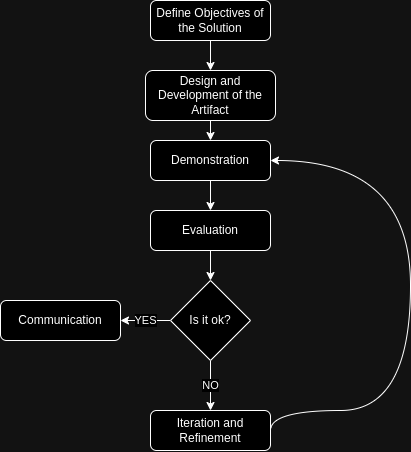
\includegraphics[width=0.7\textwidth]{assets/tools/dsr/DSR.drawio.png} % Change this to your image file
    \caption{DSR Life-cycle}
    \label{fig:sample-image} 
\end{figure}

With this in mind and better discussed further, firstly, within this work there is a definition of objectives for this solution. Secondly, there is the design and development of the artifact, which is a blockchain network. Thirdly, this network passes by a demonstration to effectively see how it behaves. Forthly, evaluations around the solution are made, and in case the solution is already good enough, communication is made; otherwise, there is once again a process of iteration and refinement that starts once again in the demonstration, creating this in a way an infinite loop until the condition of the solution satisfying the project needs is made.

%
%
%    SWOT ANALYSIS
%
%
\subsection{SWOT analysis}
\textbf{SWOT analysis} is a strategic planning tool which is often related to business. This is because it is a simple and yet powerful overviewer, that empowers organizations to set a plan for that precise moment. The acronymom \textbf{SWOT}, stands in English for \textbf{Strengths}, \textbf{Weaknesses}, \textbf{Opportunities} and \textbf{Threats}, which represent the key factors that influence the organizations success or failure. If done multiple times and by several people, it can gain multiple new perspectives that help as a decision factor because it can probably give a deeper understanding of the company competitive position, identifying potential areas for growth and also empower the staff to think better in strategies to address their challenges.
The purpose is to provide a well structured framework for decision making, which accesses internal factors like strengths and weaknesses and also external factors like opportunities and threats.
Despite it's current usage being more directed to business, it also helps in other kind of projects such as personal career planning and even research. In this project there's the intention to use it. This is because the use cases are complex, having a tool like this can help others understand the current situation, can help the stakeholders of the research to work according to the books and it can give a hint to those interested on the project to discover if it is doing well or not. 
With this in mind, there is detailed information about it further, explaining each particularity of this valuable tool.
\begin{figure}[H]
    \centering
    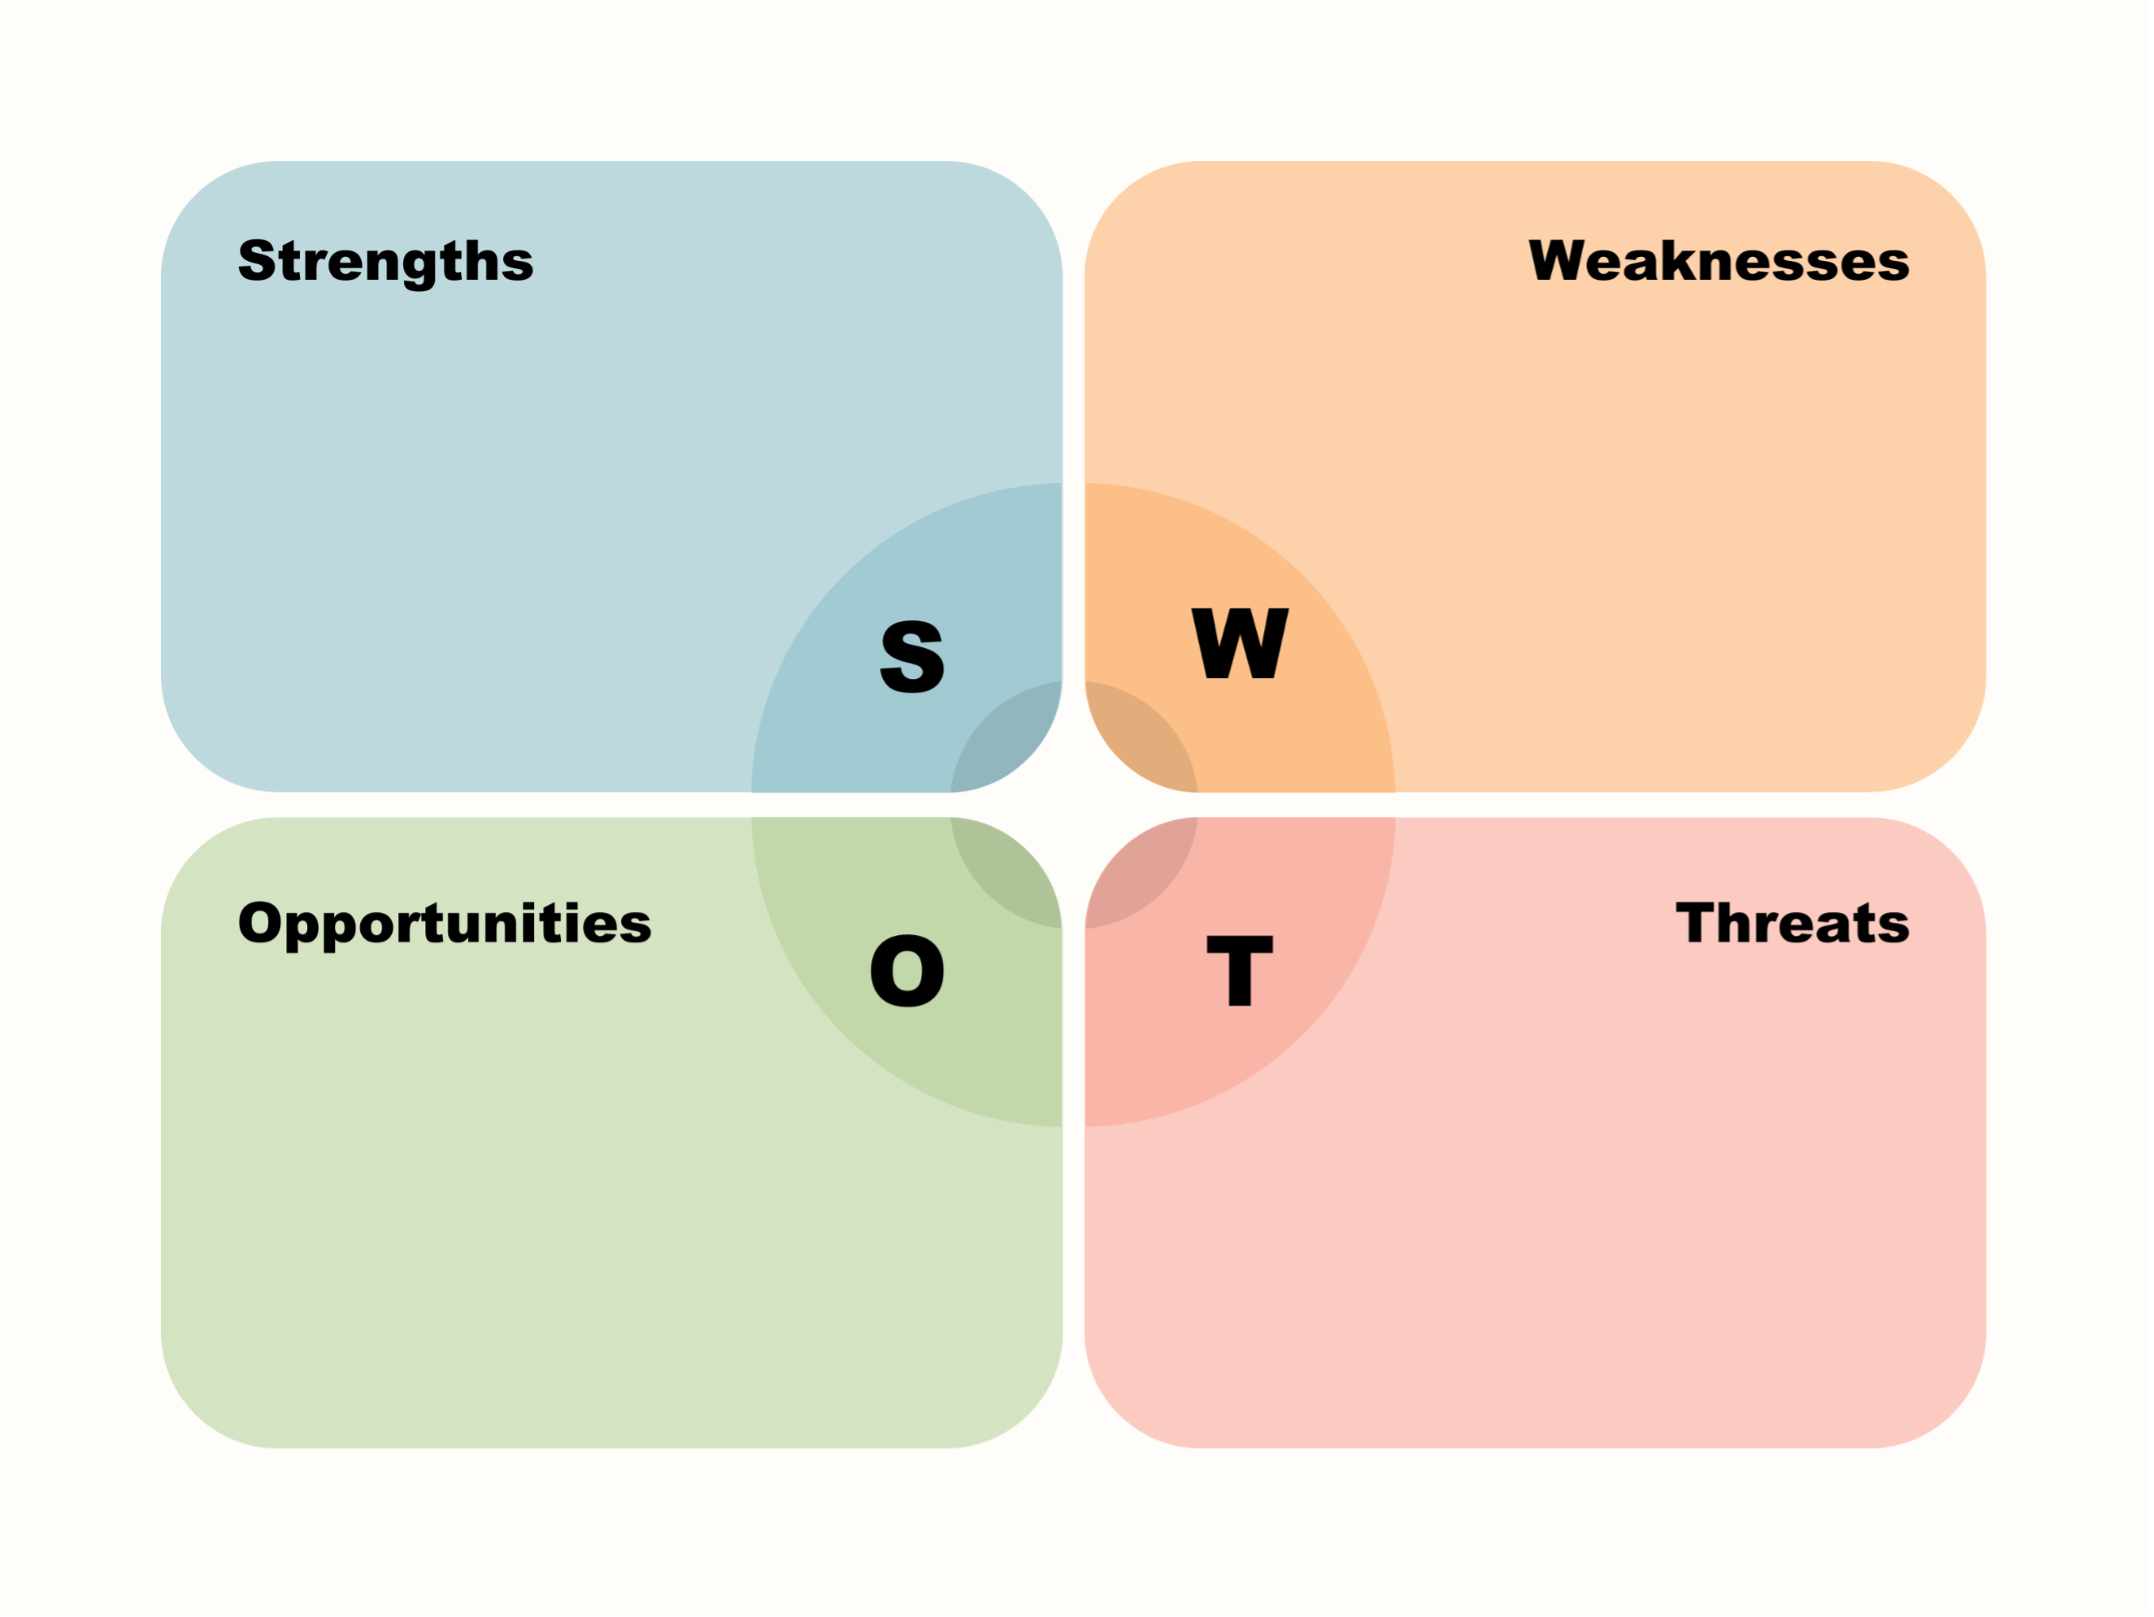
\includegraphics[width=1\textwidth]{assets/swot/SWOT.png} % Change this to your image file
    \caption{SWOT}
    \label{fig:sample-image} 
\end{figure}

\paragraph{1. Purpose of SWOT Analysis}\mbox{}\\
The purpose of \textbf{SWOT analysis} is to serve as a decision-factor for organizations. This is done by analysing internal and external factors, providing a clean environment to understand the organization competitive position and it's ability to achieve it's objectives. Putting it in more deep terms, the key purposes include:

\subparagraph{A. Strategic Planning}\mbox{}\\
To help developing strategies where the strengths will have more emphasis, weaknesses will be strengthened, opportunities exploiting will be taken and threats will be mitigated. This can be done if the organization aligns their internal strengths and weaknesses with external opportunities and threats.

\subparagraph{B. Identifying Competitive Advantage}\mbox{}\\
To outperform competitors, the organization must focus on areas where they have clear advantage. This is done by emphasizing internal strengths, such as capabilities,resources and unique advantages.

\subparagraph{C. Addressing Weaknesses}\mbox{}\\
For leaders to address challenges and reduce potential risks, \textbf{SWOT} offers insights about where the organization is vulnerable.

\subparagraph{D. Capitalizing on Opportunities}\mbox{}\\
For the recognizing and to take advantage of the market trends,technology advancements and emerging markets that could be beneficial for the growth and innovation of the organization, \textbf{SWOT} can identify the external opportunities.

\subparagraph{E. Mitigating Risks}\mbox{}\\
In order to offer risk mitigation that negatively affects the impact performance of the organization, \textbf{SWOT} offers a way to identify external threats, such as competition,regulatory changes or macro-economic downturns. This enables careful thinking about strategies that must be taken.

\subparagraph{F. Informed Decision-Making}\mbox{}\\
For developing new strategies, it is important that there is plenty of knowledge about all aspects of the internal and external environment. \textbf{SWOT} helps in this matters because, it makes sure that all aspects are considered, therefore this creates more error prone new initiatives or facilitates when it comes to enter new markets.


\paragraph{2. Internal Factors: Strengths and Weaknesses}\mbox{}\\
\begin{figure}[H]
    \centering
    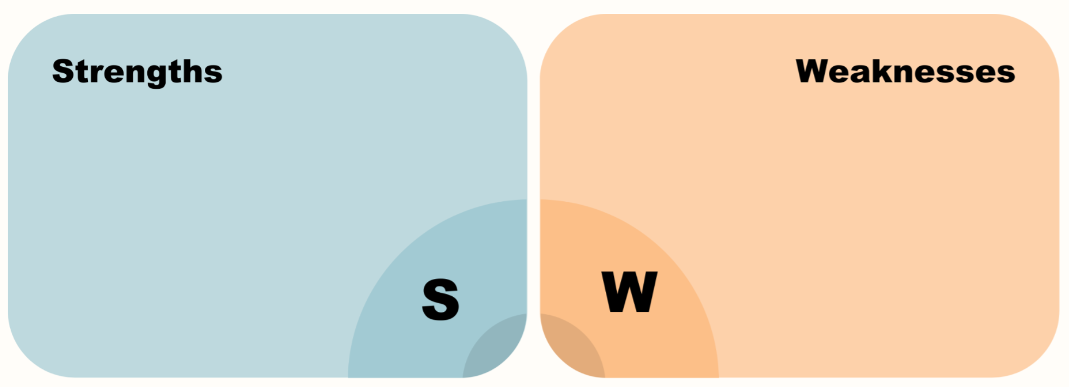
\includegraphics[width=1\textwidth]{assets/swot/strengths-and-weaknesses.png} % Change this to your image file
    \caption{SWOT: Strengths and Weaknesses}
    \label{fig:sample-image} 
\end{figure}
Representing the upper part of the \textbf{SWOT} standard visualization, there is the internal factors \textbf{Strengths} and \textbf{Weaknesses}. This is what influences the most, the ability to the achievement of the organization objectives. Understanding both strengths and weaknesses is crucial as a building block for enhancing existing capabilities and check out areas where the organization usually outperforms or the opposite. To put in other terms, the organization has the capability for control and actively manage this two, in a way where the focus is to improve but the decisions to do so are not always deterministic into that direction. With this in mind, let's make a deep dive into each to understand it further:

\subparagraph{A. Strengths}\mbox{}\\
\textbf{Strengths} are the internal contributions, so that the organization has a certain number of attributes,resources and capabilities for enterprise level competitive advantage. These are the areas or aspects where the company can outperform others, that can be used to collect opportunities and even defend against possible threats. Identifying strengths is something very valuable for organizations, because it helps in focusing on the best attributes of the organization, thereby fixing their market position.
As an example of Strengths, it could be something like: \textbf{Strong brand Reputation}, where a well established brand is widely recognized and trusted by consumers. \textbf{Skilled Workforce}, in cases where there is a qualified and experienced team who drive innovation and efficiency. \textbf{Proprietary Technology}, which are unique or patented technologies that provide a competitive edge in the market. \textbf{Operational Efficiency}, for processes and effective cost management that lead to higher profitability. \textbf{Customer Loyalty}, a loyal customer base that provides consistent revenue and positive word-of-mouth marketing and finally, more concretely for research, \textbf{Having more than enough resources}, which stands for having such resources that makes the research something more than feasible which usually is a huge challenge.
By levering this strengths, an organization can maintain or even enhance it's market position, thereby maximize its competitive advantages in relation to others, improving by extension its overall economic performance.

\subparagraph{B. Weaknesses}\mbox{}\\
\textbf{Weaknesses} are the core stone of the internal given limitations, for areas where the organization actually underperforms relatively to competitors which by extension can prevent the organization from achieving it's objectives, by representing a obstacle to the capitalization of the existing opportunities and even  by exposing the company to risks presented in external threats. \textbf{Weaknesses}, if spotted correctly, allow the organization to take measures for correctness and minimization of the impact that this unfortunate characteristics may pose in future iterations. Addressing this is essential for vulnerabilities mitigation, improve performance and prevent competitors from exploiting these causalities.
As an example, there is a lot of thinks that can be mentioned like: \textbf{Outdated Technology}, because by relying in older systems or tech can slow down processes,limit capabilities and even possibly increase costs for maintenance. \textbf{Limited Financial Resources}, where insufficient capital to invest can pose a problem to initiatives,R\&D and further expansion if desired. \textbf{Inefficient Processes}, in the idea of resource wasting, higher costs resulted from activities and delays in delivery. \textbf{Weak Brand Presence}, which represent a weakness in the essence of reduced market share and finally \textbf{High Employee Turnover}, where talent within the company is hard to maintain, thereby results in higher recruitment and training costs.

\subparagraph{C. Both combined}\mbox{}\\
By understanding and analysing \textbf{Strengths} and \textbf{Weaknesses}, there is the possibility of creating a good synergy between both which can result in organizations positioning themselves to achieve their goals. \textbf{Strengths} help creating and sustaining competitive advantages and \textbf{Weaknesses} ensures that there are no barriers for further success. In other words, considering both interchangeably will imply future success, therefore it is very important to careful think in all of those and afterwards try to see it's relations.


\paragraph{3. External Factors: Opportunities and Threats}\mbox{}\\
\begin{figure}[H]
    \centering
    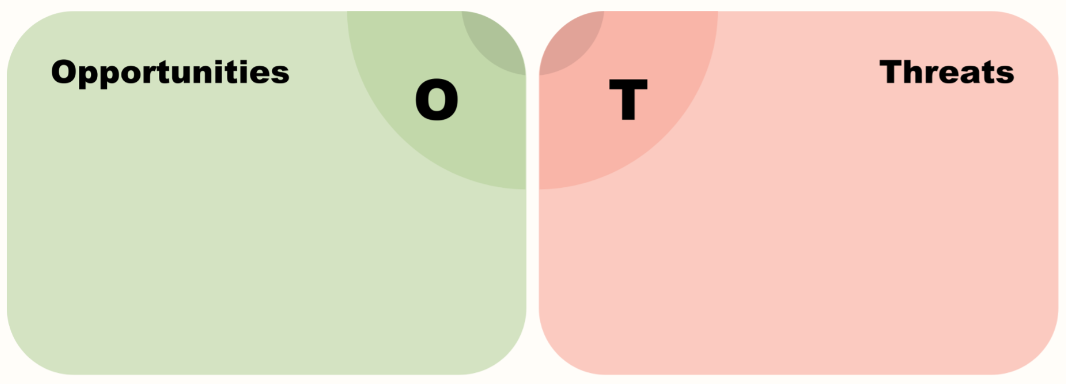
\includegraphics[width=1\textwidth]{assets/swot/opportunities-threats.png} % Change this to your image file
    \caption{SWOT: Opportunities and Threats}
    \label{fig:sample-image} 
\end{figure}
When it comes to external factors, there should be informed that those factors are the ones that the enterprise cannot control, since they don't own them and they are external to their direct manage. This means that despite the organization not being able to coordinate them, they can still take actions to make sure that those causalities don't affect them that much or that don't affect them in any way. These aspects are \textbf{Opportunities} and \textbf{Threats} and they play a huge paper in the \textbf{SWOT analysis}. Putting in different terms, those are the existences that are based in outside situations that are beyond their control, such as market trends, macro-economic indicators, competition and others. \textbf{Opportunities} provide a path for growth, while \textbf{Threats} present a potential challenge that could negatively impact the company.
A deep dive into each factor will be done in this section:

\subparagraph{A. Opportunities}\mbox{}\\
By identifying opportunities, organizations are doted of taking proactive steps toward expanding their market presence or even aggregating more into their competitive deck of cards. To achieve this, the organizations must attend to their external circumstances in order to effectively search over exploits that they can take into accordance to represent a new advantage. These, if used correctly, can help the organization grow, innovate and improve performance.
As an example, there is the following possible aspects: \textbf{Emerging Markets}, which stands for entering into a new geographic or demographic market, that offers potential for growth and expansion. \textbf{Technological Advancements}, that leverage new technologies that improve efficiency, number of product offerings or new innovative services.\textbf{Regulatory Changes}, related to new policies or regulatory shifts that if,taken into favor, can benefit substantially the organization in scope. \textbf{Shifts in Consumer Preferences}, that aims to answer to new consumer and trend behavior that can be targeted by a new product that may be on release and finally \textbf{Strategic Partnerships}, where forming alliances and collaborations with other companies can open new revenue streams.
By paying attention to opportunities, organizations can gain a competitive advantage, enter new markets and drive long-term growth.

\subparagraph{B. Threats}\mbox{}\\
\textbf{Threats} on the other hand, are challenges or risks that could affect negatively the organization. Some of these are expected, but the worst ones are those that no one is expecting and because of this there must be a lot of thoughts about it, because a lot of this comes from disguised situations. Being able to spot such things, is a important skill when it comes to project maintainability and therefore it is specially important to pay attention to, because it can be the meaning of the project ceasing and catching them early can help to take preventive measures that could minimize or even remove the effects from it. Due to the external nature, the enterprise has low control over this kind of situations but being interested in such matters, can reduce significantly the downturns.
As an example, threats can be represent as \textbf{Increased Competition}, where the increase of offering of similar products can potentially remove some market share. \textbf{Macro-economic downturns}, where the economy slows down for some reason which results in less demand for the project. \textbf{Regulatory changes}, which can result in the enterprise suffering by politics that may be against it or that revoke previous given benefits. \textbf{Changing Consumer Preferences}, that happens when the consumer shifts it's interest in the current product and benefits the competitor leaving the organization behind and \textbf{Technological Disruptions} where the advances in technology actually removes the need that the enterprise was serving, therefore making the organization service/product obsolete.
In case well informed, organizations can adapt and overcome this challenges, by preparing defensive strategies that will mitigate risks,ensure business continuity and market share protection.

\paragraph{4. How to Conduct a SWOT Analysis}\mbox{}\\
In order to come up with a \textbf{SWOT Analysis}, a systematic process of evaluating the internal and external factors is required. In other terms, the \textbf{Strengths},\textbf{Weaknesses},\textbf{Opportunities} and \textbf{Threats} are something that is in constant change, because there may be variables that were not putted into custody, new perspectives and internally or externally there is always something that may be changing because a organization is something dynamic. 
With this in mid, here's a comprehensive step-by-step guide to come up with a \textbf{SWOT}:  

\subparagraph{A. Define the Objective}\mbox{}\\
As a first step, a thematic should be specified. This makes sense since a organization is a very complex environment, thus there is a need to specify a specific matter within the company like a specific project,business decision,product launch,market entry or a specific strategic plan.

\subparagraph{B. Gather Relevant Data}\mbox{}\\
Moving to the second step, there should be collected the most data possible for gather the most important internal and external factors. These factors, based on the data can be collected through using financial reports, employee feedback and operational metrics in the case of the internal and market research,industry trends and competitor analysis in the case of the external. The data sources range from financial performance,operational efficiency,staff skills,technology and others in the case of the internal and market trends,competitor behavior, macro-economic events and customer preferences in the case of the external.

\subparagraph{C. Identify Strengths}\mbox{}\\
As a forth step, there must be a focusing in spotting the strengths. To actually get to the point where the organization can extract these strengths, a certain number of questions should be answered to carefully revise our perspectives:
\begin{enumerate}
    \item What does the organization do well?
    \item What are our unique resources or capabilities?
    \item What advantages do we have when compared to the competition?
\end{enumerate}
By answering this questions, there must be already sufficient ground to come up with actual valid answers.

\subparagraph{D. Identify Weaknesses}\mbox{}\\
In the fifth step, internal weaknesses are revised. Like mentioned before, recognizing them it's very important as other aspect of the \textbf{SWOT} but, like the threats, sometimes this weaknesses are not that easy to spot and lack of self feedback should be a barrier to come up with answers. Alike the previous step, there are questions that can help with this, being that questions the following:
\begin{enumerate}
    \item What are the areas where we need improvement?
    \item What resources are we lacking?
    \item What processes are inefficient?
\end{enumerate}
Like the previous step, the same applies when it comes to questions. By answering them there should be support enough to discussion.

\subparagraph{E. Identify Opportunities}\mbox{}\\
As a sixth step, now in the external realm, there must be answers relative to the opportunities. Likewise, but now for growth,innovation and performance exploitation, there are also a certain number of questions that could make the answer easier:
\begin{enumerate}
    \item What external trends can we capitalize on?
    \item Are there any upcoming regulations or technological advances we can take advantage of?
    \item What market gaps or consumer needs can we address?
\end{enumerate}

\subparagraph{F. Identify Threats}\mbox{}\\
In the realm of the septh step, on the other hand it comes the threats, another external factor but related to risks. These may include competitive pressures, macro-economic downturns, changes in regulations and others. Likewise again, there are a set of questions that could help with this:
\begin{enumerate}
    \item What obstacles do we face?
    \item Are there external factors that could cause problems for our business?
    \item What are our competitors doing that could threaten our market position?
\end{enumerate}

\subparagraph{G. Analyze the Results}\mbox{}\\
In the eight step and ,now that all the results were reunited, there's is plenty of capabilities to make a structured analysis. This analysis is precisely to make a correlation between all of the aspects and ,this way, play around with what could be strategies that could help in the given areas. It is important to mention that because they are related to which other, what could improve one side could make the other worst, which means that in the same proportion what could be good can actually have side effects that the organization cannot berry. 
What a organization must do in this kind of situation is: \textbf{understand how internal strengths can help on gathering opportunities} and \textbf{understand how weaknesses might expose the organization to threats}. As an example of this, in the case of the strengths to exploit opportunities there is the usage of the strong brand to expand to new markets. In the case of the weaknesses to avoid threats, in the other hand there is the update of technology to mitigate the risk of competitors offering more advanced options.

\subparagraph{H. Develop Strategic Actions}\mbox{}\\
In respect to the step eighth, this is the part where there is a creation of a given set of strategies for each element of the \textbf{SWOT}. This is challenging because they are correlated, which creates fuzz but by thinking on the effects of this strategies, bad side effects can be avoided or atleast can be taken in account.

\subparagraph{I. Review and Update Regularly}\mbox{}\\
Finally in ninth, there is a comprehensive review of what has been done so far, contributing to what was mention before with the constant change of these aspects. Either because your strategies are already making effect or simply because of the dynamic nature of a organization but the main idea here is that the \textbf{SWOT} will be continuous updated.

\paragraph{5. Applications of SWOT Analysis}\mbox{}\\
\textbf{SWOT} analysis is something that can be applied across various fields, because of it's ease of using and versatility. With this in mind, in this section, it will be delving into some of those sectors for understanding until each measure can this be useful.
\subparagraph{A. Business Strategy and Planning}\mbox{}\\
To achieve long-term objectives,grow market share and enhance competitiveness, there is a widely usage of \textbf{SWOT} by the businesses by developing and refining their strategic plans based on this. It's application ranges from \textbf{Identifying strengths to levare in competitive markets},\textbf{Addressing weaknesses to improve operations or product oferring},\textbf{Spotting opportunities for market expansion or new product development} to \textbf{Recognizing threats from competitors or economic shifts}.

\subparagraph{B. Product Development and Innovation}\mbox{}\\
To respond to shifts in customer preferences, improve existing products and introduce new products or services, the usage of \textbf{SWOT} is also relevant. It's application ranges from \textbf{Identifying product strengths (e.g., unique features, superior quality) that can differentiate it in the market},\textbf{Highlighting weaknesses such as high production costs or design flaws},\textbf{Spotting opportunities like untapped customer segments or technological innovations} to \textbf{Evaluating potential threats from competing products or changing customer demands}.
\subparagraph{C. Marketing and Brand Positioning}\mbox{}\\
To reaching target audiences,develop strategies and understand the organization brand is being positioned in the market there is also the respective usage of \textbf{SWOT}. Some of its applications in this sector are \textbf{Analyzing brand strengths such as strong customer loyalty or a high-quality product line},\textbf{Addressing marketing weaknesses, like lack of digital presence or poor brand awareness},\textbf{Identifying new marketing opportunities through social media platforms or influencer partnerships} and \textbf{Anticipating threats from new competitors or shifts in consumer preferences}.
\subparagraph{D. Competitive Analysis}\mbox{}\\
\textbf{SWOT} can be also used to comparison with other organizations. With tangible characteristics shared among them, there is the possibility to identify competitive advantages and potential areas where competitors are a actual threat to the business. It's applications are enormous in this sector like \textbf{Assessing the company's strengths relative to competitors},\textbf{Identifying weaknesses that competitors may exploit},\textbf{Evaluating opportunities in the market that competitors have not yet pursued} and \textbf{Identifying threats posed by existing or emerging competitors}.
\subparagraph{E. Project Planning and Management}\mbox{}\\
\textbf{SWOT} can also become a huge allie when it comes to project planning and management. This is because, it ensures that projects are well prepared to succeed by knowing the internal resources and external risks. More concrete applications of this are situations like \textbf{Leveraging strengths like skilled teams or efficient workflows to meet project objectives},\textbf{Identifying internal weaknesses such as limited budgets or insufficient manpower that could affect the project timeline},\textbf{Recognizing opportunities, such as new technologies or favorable market conditions that can enhance project success} and \textbf{Anticipating threats such as resource shortages, regulatory hurdles, or changing customer demands that may derail the project}.
\subparagraph{F. Risk Management}\mbox{}\\
To mitigate risks more effectively by identifying both internal weaknesses and external threats, \textbf{SWOT} can also become a good allie within this matter. This is because it identifies and addresses potential risks. 
Applications on this matter using this tool are something like \textbf{Identifying weaknesses that might expose the organization to financial or operational risks},\textbf{Analyzing external threats such as economic downturns, supply chain disruptions, or technological obsolescence},\textbf{Using strengths to build resilience against risks} and \textbf{Developing contingency plans to mitigate identified risks}.

\subparagraph{G. Personal Development and Career Planning}\mbox{}\\
In case a personal development plan is something desired, \textbf{SWOT} is a good tool to spot threats to make good career choices by spotting strengths, weaknesses and even opportunities. This means that this tool is flexible, until the point that it is not applied only to organizations but very relevant for other types of cases. Some of the applications within this concrete case are something like \textbf{Identifying personal strengths such as skills, qualifications, or experiences},\textbf{Addressing weaknesses such as skill gaps or limited experience},\textbf{Recognizing opportunities like new job openings, networking possibilities, or educational opportunities} and \textbf{Evaluating external threats like industry changes, job market competition, or economic uncertainty}.

\subparagraph{H. Nonprofit and Social Sector Strategy}\mbox{}\\
For identification of sustainability and impact opportunities and to deliver their mission, nonprofit organizatons and social enterprises also use \textbf{SWOT}. How it is applied is listed from \textbf{Evaluating internal strengths such as dedicated volunteers or unique fundraising channels},\textbf{Identifying weaknesses like limited financial resources or operational inefficiencies},\textbf{Spotting opportunities such as emerging social trends or partnerships with other organizations} to \textbf{Addressing threats such as changes in public policy, donor fatigue, or increased competition for funding}.

\paragraph{6. Advantages of SWOT Analysis}\mbox{}\\
There was been a lot of \textbf{SWOT} coverage so far. Like the purpose,it's factors,how to actually use it and its major applications. With this in mind, there will be also the coverage of its advantages in a more direct way so there is comprehensive understandability about the meaning of using such tool. Without further delay, there will be a coverage of the main ones below:

\subparagraph{A. Simplicity and Ease of Use}\mbox{}\\
The first advantage is it's ease to use, which is no surprise due to its straightforwardness. It is simple to understand therefore simple to use, making it feasible for a range of users like businesses from small to big and even for individuals.

\subparagraph{B. Comprehensive Overview }\mbox{}\\
The dual approach, internal and external section of factors,  ensures that, in a holistic way, there is coverage of all critical aspects for decision making. This is a key factor for making decisions since it gives less burden when analysing for coming up with a vision of the current state of a given project.

\subparagraph{C. Encourages Strategic Thinking}\mbox{}\\
\textbf{SWOT} creates a environment for strategic system, because it requires the organization to constantly change the aspects they have been putting into it. By constant changing, this obligates management to look beyond day-to-day operations and think more in the broader picture, focusing on long-term goals and strategies.

\subparagraph{D. Identifies Core Competencies and Areas for Improvement}\mbox{}\\
By identifying strengths and weaknesses, it helps organizations recognize their key competences and areas where they can do better, specially within the internal realm since the external realm can only be tangible through taking action from inside. This conscious, leads to a obligation for the management side to take more focused strategic decisions.

\subparagraph{E. Supports Informed Decision-Making}\mbox{}\\
For supporting data-driven decision-making, \textbf{SWOT} is widely used for revealing key insights about the organization position and the surrounding environment. This is essential for a organization to take well-informed decisions by having in their possess structured assessment of internal and external factors.

\subparagraph{F. Flexible and Versatile}\mbox{}\\
It has been proven that \textbf{SWOT} is flexible and versatile, because has it was mention before, it can be applied to a vast numerous of cases like business planning,product development,marketing,project management,risk assessment,personal career planning and even nonprofit strategy development.

\subparagraph{G. Fosters Collaboration and Team Input}\mbox{}\\
Since the data is kind of bias, having different perspectives can be a valuable insight for the organization and this is what creates a environment for comprehensive collaboration and input from the staff. By involving multiple people across the organization, \textbf{SWOT} reunites all of this insights and it helps in covering all the aspects for a well-rounded strategy for the future.

\subparagraph{H. Promotes Strategic Alignment}\mbox{}\\
Since after the last step, there is continuous monitoring of the situation and by extension mutation of the \textbf{SWOT}, alignment is expected to occur, because by having the internal and external aspects a well-coordinated strategy gets formed,  thus all get to work into the same direction.

\subparagraph{I. Risk Identification and Mitigation}\mbox{}\\
Another advantage of the \textbf{SWOT} is the prior risk detection. This is very important, due to the fact that if there are notices of deviation, organizations will develop strategies that will mitigate those risks, thereby making them prepared for challenges and uncertainties.

\subparagraph{J. Cost-Effective and Efficient}\mbox{}\\
\textbf{SWOT} is cost-effective method for evaluating business environments. This is evident, due to the fact that this analysis don't require significant financial investments or sophisticated tools like other approaches. Putting in another words, it is not expensive to use this approach and it does serve its purpose which is perform a quick and yet effective analysis of the current situation of the organization, creating means for further decision making.

\paragraph{7. Limitations of SWOT Analysis}\mbox{}\\
While \textbf{SWOT analysis} is a valuable strategic tool, it has several limitations that can affect the effectiveness of the insights. By getting to know the limitations that this tool offers, it is possible for us to delve into the realm of contra-measurements or good practises that in return can help to avoid this nuances and make a fair analyse. After deep thinking, there is below a coverage of the most relevant limitations that this framework can find:

\subparagraph{A. Lack of Prioritization}\mbox{}\\
Altought this tool reunites all of the most important information, it does not offer a structured way to prioritize them. Without a clear ranking of which factors are most critical, it becomes fuzzy for the management to take action due to the struggle of knowing which issues should be taken into custody first.

\subparagraph{B. Subjectivity}\mbox{}\\
\textbf{SWOT analysis} is unfortunately very subjective, as it relies in perspectives and opinions, which leads to a analysis. This can introduce bias or incomplete perspectives depending of the personal, leading to a vision that may not be the true representation of the organization situation. 

\subparagraph{C. Over-Simplification}\mbox{}\\
Simplicity is seen as a advantage in a lot of situations, but this becomes a burden in more complex situations where factors may not fit in the given categorizations or ,even worst, they may be a strength and a weakness at the same time.

\subparagraph{D. Static Snapshot}\mbox{}\\
Despite the \textbf{SWOT} analysis being updated frequently, they become quickly outdated in case the organization is to much dynamic, therefore, actions must be taken in order to make sure that this remains updated which is very difficult in those kind of situations.

\subparagraph{E. No Quantitative Data}\mbox{}\\
Another limitation of this tool, is the fact that the data is largely qualitative, which means that it does not contain hard data or any kind of metrics. This lack of quantitative data makes it difficult to measure significant in some points and also even more harder to establish goals which usually are better with numbers.

\subparagraph{F. Limited Actionable Insights}\mbox{}\\
\textbf{SWOT} reveals itself as limited in the actions to take, this is because it only presents a analysis and not any kind of recommendation regarding actions to take over certain situations. In other terms, the tool is limited into giving insights of the action to take in facing common problems, which means the most it can do is simply present a simple a analysis.

\subsection{Project Plan}

The following tables are conceded in respect to the activities and milestones that will be comprehended during the dissertation. It shows per month where the activity was done or is expected to be finished.

\paragraph{Activity 1 (A1)}: Literature Revision (use case 1) \mbox{}\\

\paragraph{Activity 2 (A2)}: Article (use case 1) \mbox{}\\

\paragraph{Milestone 1 (M1)}: Article Delivery to Conference (use case 1)\mbox{}\\

\paragraph{Activity 3 (A3)}: Conference Presentation (use case 1) \mbox{}\\

\paragraph{Activity 4 (A4)}: Literature Revision (use case 2) \mbox{}\\

\paragraph{Activity 5 (A5)}: Development \mbox{}\\

\paragraph{Activity 6 (A6)}: Interim Report \mbox{}\\

\paragraph{Milestone 2 (M2)}: Prototype demonstration \mbox{}\\

\paragraph{Milestone 3 (M3)}: Interim Report Delivery \mbox{}\\

\paragraph{Activity 7 (A7)}: Dissertation \mbox{}\\

\paragraph{Activity 8 (A8)}: Article (use case 2)\mbox{}\\

\paragraph{Milestone 4 (M4)}: Article Delivery (use case 2)\mbox{}\\

\paragraph{Activity 9 (A9)}: Dissertation Review\mbox{}\\

\paragraph{Milestone 5 (M5)}: Dissertation Delivery \mbox{}\\

\paragraph{Activity 10 (A10)}: Dissertation Presentation \mbox{}\\

% TABLE FOR 2023
\begin{longtable}{|c|c|c|c|c|c|c|c|c|c|}
    \hline
    & \textbf{April}& \textbf{May} & \textbf{June} & \textbf{July} & \textbf{August} & \textbf{September} & \textbf{October} & \textbf{November} & \textbf{December} \\ \hline
    
    \textbf{A1} & X & X & X & & & & & & \\ \hline

    \textbf{A2} & & X & X & & & & & & \\ \hline

    \textbf{M1} & & & X & & & & & & \\ \hline

    \textbf{A3} & & & & X & & & & & \\ \hline

    \textbf{A4} & & & & X & X & X & X & X & X \\ \hline

    \textbf{A5} & & & & & & X & X & X & X \\ \hline

    \textbf{A6} & & & & & X & X & X & X & \\ \hline
    
    \textbf{M2} & & & & & & & X & & \\ \hline
    
    \caption{Monthly plan 2023: General} \label{tab:activity_schedule} 
\end{longtable}

% TABLE FOR 2024
\begin{longtable}{| c | c | c | c | c | c | c | c | c | c |}
    \hline
    & \textbf{January} & \textbf{February} & \textbf{March} & \textbf{April} & \textbf{May} & \textbf{June} & \textbf{July} & \textbf{August} & \textbf{September}\\ \hline
    
    \textbf{A4} & X & X & X & X & X & X & X & X & X  \\ \hline
    
    \textbf{A5} & X & X & X & X & X & X & X & X & X \\ \hline

    \textbf{A6} & X & X & & & & & & &  \\ \hline
    
    \textbf{M2} & & & & X & & & & &   \\ \hline
    
    \textbf{M3} & & & X & & & & & &  \\ \hline
    
    \textbf{A7} & & & X & X & X & X & X & X & X  \\ \hline
    
    \textbf{A8} & & & & & & & X & X & X \\ \hline
    
    \caption{Monthly plan 2024: General (part 1)} \label{tab:activity_schedule} 
\end{longtable}

\begin{longtable}{| c | c | c | c |}
\hline
& \textbf{October} & \textbf{November} & \textbf{December} \\ \hline

    \textbf{A5} & X & X & X \\ \hline

    \textbf{A7} & X & X &  \\ \hline

    \textbf{A8} & X & &   \\ \hline
    
    \textbf{M4} & X & &  \\ \hline

    \textbf{A9} & & X & X \\ \hline
    
    \textbf{M5} & & & X \\ \hline
    \caption{Monthly plan 2024: General (part 2)} \label{tab:activity_schedule} 
\end{longtable}

\begin{longtable}{| c | c | c | c | c |}
\hline
& \textbf{January} & \textbf{February} & \textbf{March} & \textbf{April}\\ \hline

    \textbf{A5} & X & X & &\\ \hline

    \textbf{A9} & X & & &\\ \hline

    \textbf{M5} & & X & & \\ \hline
    
    \textbf{A10} & & & & X \\ \hline
    \caption{Monthly plan 2025: General (part 3)} \label{tab:activity_schedule} 
\end{longtable}

\subsection{Risk List}

In the following table, the risks that directly or indirectly influenced the development of this dissertation are listed. Depending on the identified risk, a mitigating action is proposed in order to minimize the impact of the risk. The scale for the Probability and Impact columns is measured from 1 to 5, where 1 corresponds to a very low risk and 5 to a very high risk.

\begin{longtable}{|c|p{3cm}|c|c|c|p{3cm}|c|} 
    
    \hline
     \textbf{Nº} & 
     \textbf{Description} & 
     \textbf{Probability(P)} & 
     \textbf{Impact(I)} & 
     \textbf{Seriety(P*I)} & 
     \textbf{Mitigation Action} & 
     \textbf{Verified}  
     \\ \hline
    \endfirsthead

    \hline
    \textbf{1} 
    & 
    Unreachable deadlines
    & 3 
    & 5 
    & 15 
    & Planning better the next events and gain experience from previous deliveries;
    & Yes 
    \\ \hline
    
    \textbf{2} 
    & 
    Requirements of the project change
    & 2 
    & 4 
    & 8 
    & Make frequent communication with stakeholder;Check well the limitations imposed by the project;
    & No
    \\ \hline

    \textbf{3} 
    & 
    Lack of Time
    & 4 
    & 5 
    & 20 
    & Implement only what is actually needed
    & Yes
    \\ \hline

     \textbf{4} 
    & 
    Resources
    & 4 
    & 5 
    & 20 
    & There are no mitigation measures
    & Yes
    \\ \hline

     \textbf{5} 
    & 
    Incorrect understanding of data
    & 2 
    & 5 
    & 10 
    & Spend more time analyzing the data; Make sure that the data is relevant for the object of study;
    & Yes
    \\ \hline

    \textbf{6} 
    & 
    Mistakes
    & 1 
    & 5 
    & 5 
    & Don't do tasks in automate mode; Focus more in the tasks;
    & Yes
    \\ \hline

    \textbf{6} 
    & 
    Security implications
    & 1 
    & 5 
    & 5 
    & Follow standards; Try to learn more as the time passes;
    & No
    \\ \hline

    \textbf{7} 
    & 
    Complexity of the project
    & 2 
    & 3 
    & 6 
    & Document Everything; Simplify everything;Join Communities;
    & Yes
    \\ \hline

    \textbf{8} 
    & 
    Unknown Errors
    & 2 
    & 4 
    & 8 
    & Join Communities;Arrange more debug mechanisms;
    & Yes
    \\ \hline

    \textbf{9} 
    & 
    Acceptance
    & 4 
    & 5 
    & 5 
    & Make the best solution possible;Make clear the need of the solution;
    & No
    \\ \hline

    \caption{Risk List: General} \label{tab:activity_schedule} 

\end{longtable}

\subsection{Relevant tools}

Before delving into the use cases and what was done in practical terms, there is a need to explain seamlessly which tools were used during the project. This is because, by explaining what was used, by extension, an assumption by the reader for the reason why certain things were inserted in the project is achieved. Some tools are related to blockchain, since that is the main subject under scrutiny along with the healthcare sector, but others, on the other hand, are extensions of a product that is strong by itself. Reasons for the usage of blockchain were already mentioned in the State of Art; thereby, there is no reason to go much deeper in this aspect, but returning to the other tools, they are needed for commodity purposes, and probable risks resulted by the usage of certain tools will be covered further in this thesis. Also, it is important to mention that the idea around this project is not to achieve excellence in decentralization, to simply use emergent technologies because they are trendy, but to try to solve the existing problems with the best set of tools that are proven to be the best in the current market and perhaps standardize the way private blockchains are designed to gain broad acceptance. Standardization helps with broad acceptance because this way implementations are not that fuzzy like they were before, contributing to ease in implementations and creating a common path between people that, in case of obstacles, there may be a current solution already because someone crossed the same path before. This is essential for a vast spread adoption, and thereby that's our contribution here.
There are 3 covered sections within the tools; the list is not at all complete, but there is an effort to cover the most important concepts of technologies that were used during the project. This will empower the reader with the correct view of what has been done so far.
There is a Microservices section in which the tools are a part of the other tools that will be covered. They retain an honored representation on this project because their usage is meant to empower administrators with capabilities such as resource management, easier setup of networks, decoupled services, scalability, and high availability.
Another important section is analytics; this is very important for any type of robust system, and its aim does not reside only in maintainability. It empowers the project with also mechanisms to detect bottlenecks, detect unexpected behavior, troubleshooting support, debug support, benchmarking, observability, measures to better resource management, and more.

Finally, there is also the web development section, which is used in this project as the core to build extra services that may be required for the normal function of the network. They work mostly for communication support, for ensuring security, and to help automate procedures during the results obtained in this research, but also for future usage while using this in a real environment.


\subsubsection{Blockchain}
This section will contain all necessary related or close related information about blockchain that is being used in this research. The aim in this section is to give a good fundamental overview about \textbf{Hyperledger Fabric}, the private blockchain technology that is used all over the investigation and also to give some hints about \textbf{IPFS}, which despite not categorized as a blockchain, has a lot of characteristics that resemble a blockchain thereby despite the section name, it still makes sense to put it here for the purely sake of relation between the concepts making it easier to digest. The first is considered a general purpose technology, which can be used with all kinds of data but having the capability of working with all kinds of data and at the same time be capable of dealing with all types in a effective way that's a completely different story and, because of this and also to respect to files, there was a need to think in a extension of the blockchain capabilities where \textbf{IPFS} can effectively play its rule. Altought intriguing, in this work there was not a measurement of performance regarding this technology and how it would behave in the private landscape, which means that atleast in this realm there are no tangible evidence of effectiveness on our side, which may result in the future measurements while working interchangeably with both the blockchain and this technology for storing files, exacly like describe in one of our future mentioned use cases.

\paragraph{3.5.1.1- Hyperledger Fabric}\mbox{}\\
To understand \textbf{HLF} (Hyperledger Fabric), there must be an understandable view of what a blockchain is. In an abstract way, this concept refers to an immutable ledger maintained within a distributed network of peer nodes. Each node maintains a copy of the ledger by applying the same logic to their ledger. If all reach the same result, this view of the world becomes valid, and everyone gets to keep the same state. The process mentioned here is thereby called \textbf{consensus}, which is a protocol where there is a validation of blocks that inside contain these tasks that must be endorsed by a collective number of nodes. To actually reach the point where the block is validated, all of it's transactions must be accepted by a number of nodes that depends on the configuration of the network. If a transaction gets no validation, this transaction is not included in the state of the ledger, which means it is not valid.

The first and most widely used cases of this are \textbf{Bitcoin} and \textbf{Ethereum}. Both serve different but related purposes; both fall into the class of blockchain, but these ones are public ones, like mentioned in the state of the art of this thesis.

As the popularity of these 2 plumed, other derived technologies coming from the same concept started to emerge. With this in mind, a more enterprise-friendly approach started to grow, though many organizations still need performance characteristics that presently permissionless blockchain technologies are unable to satisfy. Also, there are other requirements that also present a challenge for this approach, which are: the requirement of identity for financial transactions where \textbf{Know-Your-Customer} (KYC) is required and \textbf{Anti-Money Laundering} (AML) regulations; networks need to be permissioned; high transaction throughput performance; low latency of transaction confirmation; privacy; and confidentiality. \textbf{Hyperledger} was literally designed to meet these precise characteristics, not needing to adapt like other solutions, and that's what differentiates it from others.

\textbf{Fabric} is an open source permissioned distributed ledger platform designed for use in enterprise contexts, delivering a certain number of capabilities that are imperative in business scenarios. It is maintained by the \textbf{Linux Foundation}, and it presents an architecture that is modular and also configurable. It supports smart contracts through general purpose programming languages like \textbf{Go}, is permissioned, has pluggable consensus protocols that range from existing default ones to custom, does not require a native cryptocurrency, and offers one of the better performing platforms today of this kind for transaction processing and transaction confirmation latency.

This framework will be intensively used in the provided use cases. With this in mind, this section will be a solid coverage all over the main concepts of this framework.

Relatively to \textbf{Permissioned Networks}, this is a concept relative to a type of blockchain. Dissimilar to public blockchains such as \textbf{Bitcoin} and \textbf{Ethereum}, often called \textbf{permissionless} blockchains, these ones restrict access to a set of known participants, making them ideal for applications that require trust and control over the membership. Like mentioned before, \textbf{Hyperledger fabric} is one of these types, and so is \textbf{Corda}. Both platforms emphasize accountability without relying on a central authority, enabling organizations to construct custom and heterogeneous applications where there is a clear conscience of who can participate in the network \cite{permissioned-blockchains}. Usually, the usage of one restricts the usage of the other.However, there are also approaches where networks may want both \textbf{permissionless} and \textbf{permissioned}, referred to as \textbf{two-tier blockchain}, where both types are combined to allow both participation and validation, such as supply chain or cross-border financial transactions \cite{two-tier-permission-blockchains}. For the context of healthcare, \textbf{permissioned} is obviously more appealing, such that \textbf{operational efficiency} and \textbf{transaction security} when combined with restricted trust between participants is needed for \textbf{security} and data \textbf{privacy} \cite{permissioned-vs-permissionless-tradeoffs}.

Furthermore, there is also the modularity of \textbf{Hyperledger fabric} to be covered. It has 5 components: the \textbf{Peer},, \textbf{Orderer}, \textbf{Chaincode}, \textbf{Ledger}, \textbf{CA's (Central Authorities)}, and \textbf{client}. Each component will be covered with more extension in this category.

\begin{figure}[H]
    \centering
    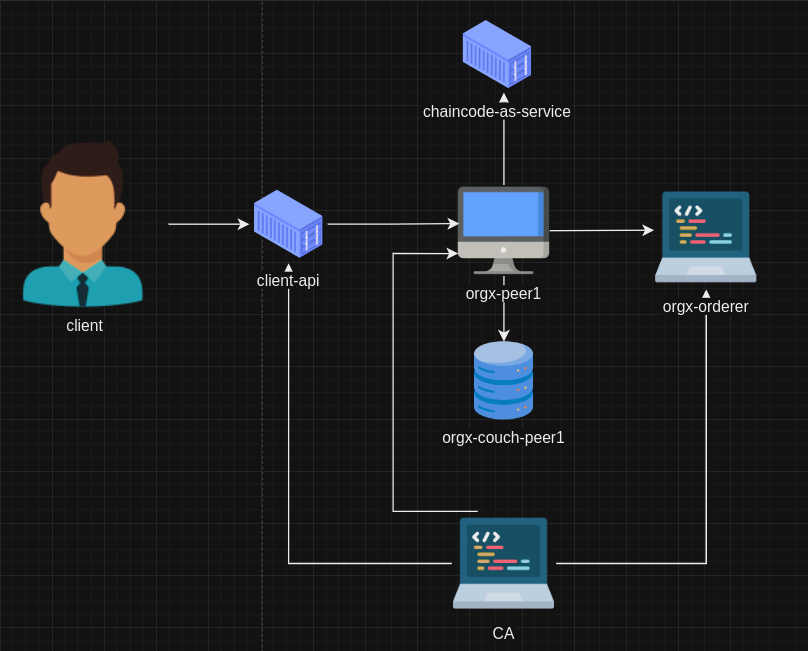
\includegraphics[width=0.8\textwidth]{assets/tools/hyperledger/hlf-minimal-setup.png} % Change this to your image file
    \caption{Major components Relationship}
    \label{fig:sample-image} 
\end{figure}

As an overview above, there is an image that illustrates not the communications but how components may relate with each other. Also, it should be noted that this is very far from representing a whole system, where usually multiple peers must endorse transactions and multiple orderers must order transactions and blocks. Putting in another terms, the representation here explained is just for the sake of understanding how individual components work with each other. With this in mind, each component's individual functions will be covered more ahead.

The \textbf{Peer} (orgx-peer1) in this representation is the middle point of everything. This is because it is the one that receives the transaction proposals and endorsements that come from other peers by previous request of a client. It also receives blocks from the \textbf{orderer}, and it is responsible for endorsement of transactions by using the \textbf{chaincode}, and furthermore, after validation through this \textbf{endorsements}, it is the one that receives a \text{block} containing valid transactions from the \text{orderer} (orgx-orderer), for then to include in it's \text{ledger} (orgx-couch-peer1). The \textbf{client}, on the other hand, manifests in two ways: the client itself as an actor and the \textbf{client-api}, which turns out to be the application itself that is responsible for calling the \textbf{Peer}. The \textbf{chaincode} (chaincode-as-service) simply runs logic, which is what the \textbf{Peer} endorses, by running the application against the \textbf{ledger} (orgx-couch-peer1). In respect to the \textbf{ledger}, it is used as a mock to endorse transactions to see if the output is the same within the vast majority of peers.The \textbf{orderer} receives transactions and puts them inside of blocks, and after ordering these transactions and blocks, it delivers the blocks to the peers. Finally, the \textbf{CA}(certificate central authority) only gives cryptographic materials so that components can identify themselves within the network. It must be known as well that the chaincode-as-a-service has the option to create TLS connections with the peer. In this picture there is only one CA for purposes of simplicity on this explanation, because usually there can be a chain of CA's and in each level, for purposes of good practices, should have 2 CA's where one is for normal certificates and the other is for TLS. The difference between normal and TLS certificates is that one is for identification and the other is to secure the communications with encryption. Once again, in this representation only normal certificates are considered, but within the network there are both, which contribute to a secure environment. \cite{rfc5280}.Now that their relations were described, let's describe them in more deep terms for further explanation.

In what concerns the \textbf{peer}, this is a fundamental concept within the network since it is responsible for managing \textbf{ledgers}, \textbf{smart contracts}, \textbf{transaction proposals}, and \textbf{endorsements}. \textbf{Ledgers} and \textbf{Smart contracts} will be explained further, but a transaction proposal is a transaction that was signed by some entity that wants to be further endorsed by the peers for then to be included in the ledger if valid. \textbf{Endorsements}, on the other hand, are the process of a peer running the logic within the proposal against its ledger. Depending on the configuration of the channel and the number of peers that validated this proposal, this transaction will be included on the block or not (within the orderer side); therefore, it could be or not included in the ledger depending on its validity.

In the \textbf{Orderer} sphere, however, there is the responsibility of receiving endorsed transactions, which, depending on the number of signatures of the peers in it, could add the transaction to a block or reject it. In the case of the first, after ordering the transactions and the given blocks, it returns to all the peers this given block. Block this that will be used for the peer to insert its operations against its ledger, therefore ensuring that every single peer has the same view of the state because they are all running the same operations against the same state. To achieve this, the orderer uses what is called a \textbf{consensus protocol}. This protocol is a mechanism to reach agreement in the sequence of transactions, but that will be discussed further.

Another vital pillar for the network is the \textbf{Smart contracts}, more commonly called \textbf{Chaincode}. This is where all of the business logic runs, and it uses abstractions to communicate with the ledger. Usually, installation is required only once. However, it must be added per channel if that is the intention of the participants within that channel. This means that I can have the chaincode installed, but this chaincode could potentially not be allowed to be called because, for that, it must be proposed to be added and committed when a certain number of participants agree on its insertion. Besides that, there are 2 typologies for usage of chaincode: \textbf{normal chaincode installation}, which occurs per peer and the chaincode becomes more like a side container, and \textbf{chaincode as a service}, where the chaincode becomes a service and to install it there must be passed metadata for the connection management. The normal way is often used for questions of ease, and, along with it, there is the certainty that the chaincode that is being invoked is in fact the desired one, since it is literally a side container or side service of the peer, therefore also giving more isolation to it. The other way, however, depending on how it is deployed, it can be reused by multiple peers, which means that if an operator does not retain this service within its infrastructure, it may represent a risk since the endpoint could be the same and its application could be changed. Be mindful that, in case the \textbf{chaincode as a service} is adopted, depending on how it is implemented, it can be exposed to the common microservices vulnerabilities, and further actions should be taken to prevent these \cite{microservices-common-vulnerabilities}.

\textbf{Ledger}, on the other hand, is a normal database like \textbf{couchdb} \cite{couchdb}. This is the state that the \textbf{Peer} uses as a mock to run its business logic and get an output for later usage for the endorsement procedure. Transactions can be rejected by either violating some business logic or by presenting different outputs among the peers. As an example, let's suppose there are 3 peers. In the first situation, peer 1 rejects the transaction because the business logic says so. The other 2 peers, peer2 and peer3, respectively, accept the transaction. In the case of a majority policy, the state resulted in peer2 and peer3 being included in peer1 as well, simply because the majority wins. Also, let's consider the case where peer 1, peer 2, and peer 3 have different outputs, but the signatures were still reunited because the transaction was not rejected. What will happen is that when this transaction reaches the orderers, the orderers will reject its validity. This is because, despite passing the peer endorsement, the orderer endorsement will fail due to a lack of determinism between the three peers. Also, within the same database, there could be different slices of data for each \textbf{channel}. However, the concept of channel is something that should be delved deeper into more ahead.

Speaking about \textbf{CA's}(Certificate Central Authorities). This is a service that serves cryptographic material like private keys and x509 certificates, which within a \textbf{hyperledger fabric} network form a \textbf{MSP} (Membership Service Provider). \textbf{MSP} is a mechanism designed for providing a way to offer identities that could be trusted and recognized by the rest of the network. To achieve this, there is the usage of this cryptographic material provided by the CA's where a key pair is offered. One of these pairs, the private key, is used to sign transactions, and the other, which is public, gets shared among the entities that will be communicating with the owner of the private, giving them a way to verify that this signature is actually valid. \textbf{Hyperledger} lets the operator either rely on existing public CA's, use their CA implementation, or simply use a \textbf{hybrid} methodology. The main difference between the public and their implementation is that it's implementation already comes with a given file structure to make the configurations easier and also the aggregation of more responsibility to the operator, but that's something that is not the concern here, thereby it should not be extended.

Relatively to the \textbf{client} within the hyperledger fabric components sphere, there is a close relation in
how it operates with the chaincode. Like chaincode, both can be implemented with a certain number of
high-level programming languages such as \textbf{Go}. Both use an interface, attributed to their set of tasks in aim.
In the case of the \textbf{chaincode}, its interfaces are related to making interactions with the ledger, but in the case
of the client, its abstractions are focused on making calls against the peer by giving metadata related to
the \textbf{channel} and methods to be targeted. Thus, it’s more formal name is \textbf{Fabric SDK}, where there is the
opportunity to use \textbf{Node.js}, \textbf{Java}, and \textbf{Go}. Giving the opportunity to perform various functions, such as
creating \textbf{channels}, submitting \textbf{transactions}, querying the \textbf{ledger}, and managing the \textbf{chaincode}. Within
the \textbf{SDK} ,there are various subpackages aimed at serving different purposes, like: \textbf{gateway}, for establishing
connections to the network and provide access to \textbf{channels} and \textbf{contracts}. \textbf{Network}, which represents
a channel that a client can interact with. \textbf{Contract}, conceded for iteration with a given smart contract
deployed in a \textbf{channel}, used for submitting and evaluating transactions, and finally Wallet, responsible for
managing user identities and credentials for connecting to the \textbf{fabric network}. Further details should be
seeked within the proper documentation of \textbf{hyperledger fabric}.

Besides all of this, there are also a certain number of extra topics that should be covered for an extensive understanding of \textbf{hyperledger fabric}. This topics are, more in depth, \textbf{Consensus Mechanism},\textbf{Privacy and Data Confidentiality},\textbf{Channels},\textbf{Scalability},\textbf{Endorsement Policies},\textbf{Governance and Membership Services},\textbf{Real-World Use Cases} and also \textbf{Importance in this project}.

Starting with the \textbf{Consensus Mechanism}. This is a protocol that originated within the context of distributed systems. The most well-known protocol is \textbf{Paxos}. Although not implemented in the context of \textbf{hyperledger fabric}, it is of high importance to refer to it. This is because this algorithm was the first and major one of them all, contributing to the creation of further, simpler, and well-designed algorithms. For reference, \textbf{Paxos} is a consensus algorithm that originated for achieving agreement between a network of unreliable nodes. It was introduced by \textbf{Leslie Lamport} in a series of papers, starting with \textbf{The Part-Time Parliament} in 1988 \cite{paxos-main} \cite{paxos-simple}. It's importance comes from ensuring that a vast number of nodes can agree on a single value, even in the presence of network delays, node failures, and other types of faults. Also, it was the building block of major projects such as \textbf{Google's Spanner}, \textbf{Amazon's DynamoDB}, and \textbf{Apache ZooKeeper} \cite{google-spanner} \cite{zookeeper} \cite{dynamodb}. It is considered a building block precisely because, like other algorithms, every single one of these projects has its own implementation according to their use case, which means that all are deviations of the original \textbf{Paxos}. However, although very powerful, it has begun to become more obsolete because of its complexity. Putting in another words, though very powerful, it is hard to understand, thereby hard to implement, and by extension, hard to debug or resolve issues, not speaking about other major concerns such as \textbf{Performance} due to it's reliance on multiple phases and need for communication with the majority of nodes and also because of its \textbf{Scalability} problems, where this algorithm requires a huge number of message passing, therefore causing an overhead in the network.

Deviating from \textbf{Paxos}, other algorithms surge, such as \textbf{PoW},\textbf{Kafka},\textbf{Raft} and more recently \textbf{PBFT}.

Speaking of \textbf{PoW}(Proof of Work), this algorithm is well known for serving decentralized networks like \textbf{Bitcoin}. However, there are implementations of this protocol under the \textbf{Hyperledger fabric} umbrella, which means that it's practical cases are not just suited for public implementations alone. It's conception exists around solving complex computational puzzles that require significant effort to complete, but at the same time very easy to verify \cite{PoW} \cite{PoW-hyperledger} \cite{pow-hibrid-hyperledger}.

In second, it's worth to mention \textbf{Kafka}, more well known in the hyperledger community as \textbf{crash fault-tolerant}(CFT) consensus mechanism for ordering transactions. This one got replaced by \textbf{Raft}, which is simpler and will be covered next. CFT is an algorithm that uses \textbf{Apache Kafka} in combination with \textbf{Apache ZooKeeper} to establish an ordering service that provides total ordering of transactions in a permissioned blockchain network. \textbf{Kafka}, with its publish-subscribe messaging system designed for high throughput and fault tolerance, was doing the handling of message ordering and durability by putting the messages into topics and partitions, while Zookeeper was used to manage Kafka brokers, ensuring that Kafka partitions are assigned to brokers, and was also helping in tasks such as leader election \cite{kafka-consensus}.

In third, there is the mention of \textbf{Raft}. This is the current most-used consensus algorithm, and it's very claimed by its simplicity, giving the same results as Paxos. To achieve this, raft elects a leader among a group of distributed nodes, ensuring that all nodes agree on the same sequence of operations. More concretely, when a leader ceases to exist, every node enters a random timer state where the first peer to send its vote request message usually becomes the leader. This is because the others, by receiving this request, enter a non-candidate state since there is a peer who requested it first. After reuniting the majority of votes, and since each node can only vote once, this node becomes the leader, and every log replication passes by him to endorse. With this, log replication is guaranteed, creating safety and consistency within the network. By offering simplicity and robustness to a distributed system that requires replication, \textbf{Raft} has become the most broadly accepted consensus algorithm, having implementations such as \textbf{etcd} and \textbf{Consul} \cite{raft-consensus} \cite{etcd} \cite{consul}.

Lastly, in terms of consensus algorithm, it surges the most spoken one lately, \textbf{PBFT}(Practical Byzantine Fault Tolerance). This algorithm was introduced by Miguel Castro and Barbara Liskov in 1999 and is widely used in permissioned blockchain networks. Although it is older, it has only been implemented in \textbf{Hyperledger fabric} now, and it promises to get rid of faulty or even malicious nodes. \textbf{PBFT} can tolerate up to (n-1)/3 faulty nodes in a network of n nodes by using a \textbf{Three-Phase Commit} approach. Despite it's enormous advantages like \textbf{High Fault Tolerance}, \textbf{Low Latency}, and \textbf{Deterministic Finality}, it still comes with disadvantages like \textbf{High Communication Overhead} and \textbf{Leader-Based approaches} \cite{pbft}.

Changing headlines, \textbf{Privacy} and \textbf{Confidentiality} are critical components of information security and data protection strategies. \textbf{Privacy} refers to the right of individuals to control their personal information. This is done by giving the power of control over how it is collected, stored, and shared. It is about ensuring that personal data is not shared or used without people's consent.  On the other hand, there is \textbf{Confidentiality} which proves to be about the protection of a user's data from malicious, non-desired access, making sure this way that the information remains available only for those that were allowed to have such. In the healthcare context, it is required compliance against the \textbf{Health Insurance Portability and Accountability Act (HIPAA)} and \textbf{General Data Protection Regulation (GDPR)} \cite{hipaa} \cite{gdpr}. Also, \textbf{Hyperledger fabric} helps achieving these regulations by offering characteristics such as \textbf{Permission Blockchain Model},\textbf{Data Privacy Through Channels},\textbf{Data Confidentiality With Private Data Collections},\textbf{Access Control and Identity Management},\textbf{Auditable Data Sharing and Provenance}, and \textbf{Data Encryption and Secure Data Sharing}. Firstly, \textbf{Permission Blockchain Model} helps to fit in the regulation because it offers a network where all participants must be authorized and well known. Secondly, \textbf{Data Privacy Through Channels} is also another characteristic that does fill the needs of regulations because \textbf{channels} enable private communication between a subset of participants, where each channel has its own segregated ledger. Thirdly, \textbf{Data Confidentiality With Private Data Collections} also helps on this because Hyperledger can create private collections within a channel that, despite still fitting in the main ledger, are privately only available for a set of given participants. Fourthly,\textbf{Access Control and Identity Management}, because \textbf{Hyperledger} uses the \textbf{MSP}(Membership Service Provider), managing effectively the roles within the network, creating fine-grained access control, and enabling authorized access to resources. In fithly, there is the concept of \textbf{Auditable Data Sharing and Provenance}, due to its offering of logging records, making audit easier; thereby, it complies with \textbf{GDPR}, and like mentioned before, due to the providing of a history of events, it shows clearly how records are being managed, spotting probable malicious activity and identifying the bad actor if needed. Finally, \textbf{Data Encryption and Secure Data Sharing}, since it allows encryption of data, ensuring that the data is protected against malicious access \cite{privacy-hlf}.

Apart from what has been covered so far, there is the concept of \textbf{channel}. This concept is very important since it is the existing mechanism that allows you to aggregate a certain number of components, thereby creating a linkage between them and a precise section for them to exchange information. Within the documentation of \textbf{Hyperledger Fabric}, there is the reference to channel as a \textbf{group of friends}. This is because, exactly like a channel, you have multiple groups of friends on your social media, and their members are different depending on the task or the theme to be discussed within that group. Also, within those groups there is an exchange of information that is private and it's not shared with other group members, which is essentially the same thing as a channel. In a channel, you aggregate a certain number of components that could be part of multiple different organizations depending on what you want to be sharing within that channel, and also within this channel, there is the option to create a \textbf{private collection}. Despite the theme being the same, there are participants that may want to discuss information regarding this discussion within the group but just with a set of participants, especially like it would be with the private collection. Though the difference with a friend group is the nature of blockchain. This means that with a private collection, there is the option of creating a subset within the channel, making others able to see that you are communicating with each other but not what they are exchanging. In other terms, a given organization can be in multiple channels, with multiple different individuals in each, and it can also create multiple private conversations regarding the same theme, but just with a subset of participants in the same channel and exclusively of that precise channel. As an example, let's think of an organization that has the idea of creating a group of medicament's suppliers and other group of medical clinical reports. Obviously, in these examples, there will not be common participants because their nature is different. The organization may discuss within that group that it needs medicaments for X. Supposing they want to buy the cheapest one, they will request it from the enterprise Y. This enterprise, although offering it more cheaply, may not have the quantity to satisfy this need, making this organization forced to go to supplier Z to satisfy the rest of the demand. Maybe, for the benefit of this organization, prices of the product should not be known by the participants within this channel, which means that at least the monetary transactions within this channel should be done in private collections. However, the transactions of products could be done publicly, therefore making it easier for all of the participants to have the information publicly available that this organization is supplying itself from these two organizations, making others in the obligation of trying to bargain to also benefit from this channel. Also, the same applies to the clinical registry, even if it has a different logic or idea. There may be information that can be publicly exchanged between doctors, but there may also be communication that should only be sent within a more restricted set of individuals within that consortium. With channels and private collections, hyperledger obtains data confidentiality,selective data sharing and regulatory compliance \cite{private-collections}. 

Delving into the \textbf{scalability}, this is most concerned matter when it comes to the \textbf{blockchain}. Since this is a complex environment to maintain, various factors could potentially harm the performance of such, making it infeasible as a project if not taken into account the following factors that could affect it: \textbf{consensus mechanisms},\textbf{network size}, and \textbf{network configurations}. \textbf{Consensus Mechanisms} could be a problem because there are certain algorithms in consensus that offer more fault provenance but at the same time lose performance because of the number of operations to achieve a more secured consensus, making it, like mentioned, more fault provenance but at the same time slower. There are works concerning the comparison of such \cite{consensus-performance}. \textbf{Network size}, on the other hand can be also a problem to the performance, because when it comes to the blockchain, having a bigger network means more nodes to achieve consensus, therefore causing the network to be slower do to all the communications required to reach the consensus. To address this, there are techniques to make the consensus faster, like side chains or sharding, consisting of making the consensus within a subset of peers, not implying that the whole network reaches a consensus but that a subset does,therefore making the network faster \cite{sharding}\cite{side-chains}.Finally, \textbf{network configurations} is related more to settings that are presented in various domains of the blockchain. There are enormous parameters that could be settled within the hyperledger landscape. This parameter is categorized by its own domain presence, and changing them could benefit or make the performance worse, but keep in mind that, in order to do that, there is the requirement of understanding the particularities of each deeply; otherwise, changing the default values could imply problems in the future. As an example, there are the categories \textbf{Block Size} and \textbf{Consensus Settings}.  In the \textbf{Block Size} sphere and, without mentioning everyone, there are settings such as \textbf{MaxMessageCount} for a max number of transactions within a block and \textbf{AbsoluteMaxBytes} for the maximum size of a block in bytes. In the \textbf{Consensus settings}, on other perspectives and also without mentioning everyone, and in the case of the \textbf{Raft} protocol, there can be found settings like \textbf{Heartbeat Timeout} for heartbeat messages to followers interval and \textbf{Snapshot interval} for the interval for which there is the need to make snapshots of the current logs \cite{changing-hlf-settings}.

\textbf {Endorsement Policies} are another big dinosaur in the room when speaking about \textbf{hyperledger fabric}. These are the rules under which the transactions will need to apply, making the transactions valid in case they succeed and invalid in case they fail to do so. In other terms, these are the policies that define which peers must sign (endorse) a transaction before it can be valid and aggregated to a block by an orderer. It specifies how many and which organizations must approve the transaction before it can be inserted into the ledger.

Piercing to the real use cases realm, there are several occurrences of hyperledger appliances. The sectors affected by this remarkable technology were: \textbf{Financial},\textbf{Healthcare},\textbf{Supply chain management},\textbf{Goverment and Public Sector}, and \textbf{Insurance}. Within the \textbf{Financial}, various banking consortiums were created for processing cross-border payments, managing the financial chain, and enabling transparent asset transfers \cite{finances-use-case}. In the \textbf{Healthcare} there are also a lot of occurrences of it's usage for managing electronic health records (EHR's), which is possible due to the channels and private collection capabilities, allowing sharing of patient data between healthcare providers \cite{healthcare-use-case}. In the \textbf{Supply chain management}, there are multiple occurrences for the usage of hyperledger fabric for tracking goods. By using this, enterprises were dotted of track food products from the farm until the shelf, reducing the time required to trace the origin of food products in the event of contamination while still offering privacy for sensitive business data using private collections \cite{supply-chain-use-case}. Also, when it comes to \textbf{Government and Public Sector}, it is well known that there are already present in the market implementations for the usage of such technology for managing digital identities, land registries, and transparent voting systems \cite{public-sector-use-case}. Finally, there is the usage for \textbf{Insurance}, where there are retained implementations that are meant to help claiming processing and reduce fraud. Thus, by levering this, the \textbf{Insurance} can collaborate in a shared ledger to verify these claims and manage shared data, reducing duplicated and fraudulent claims \cite{insurance-use-case}.

As a final for this section, the \textbf{importance} of this tool for this thesis must also be explained. As it has been explained, this technology is very complex; there are a lot of alternatives for it; it's emergent, and there are still problems that must be addressed. However, the urge to choose it over others's comes from the community that it has, the current and continuous work that is being released over it, the fact that it is being used by the major companies such as \textbf{IBM}, its modularity, and it's already uncovered advantages within the healthcare sector. This is the aim of the research, which makes it a more favorable choice for the project; therefore, the use cases that will be crossed further will be both based on this.

\paragraph{3.5.1.2- Ipfs}\mbox{}\\
When it comes to \textbf{IPFS}, it must be known that this does not represent a blockchain, though its concepts derive from a P2P perspective, which means there are relations between the two. It is a modular suite of protocols for organizing and transferring data \cite{ipfs}.

More concretely,\textbf{IPFS} is a tool that stands for Interplanetary File System, where it refers to an implementation that was meant to become the file system of the future.

Their aim is to serve as a decentralized file system where, to achieve that, what is required is having a distributed system that goes through an immense decentralized network of heterogeneous numbers of peers. This way, by adding a file or an image, there will be a unique identifier for that file. In the case of that file being a folder, it generates an identifier for himself and for the respective children's and stores it in an \textbf{DHT} (Distributed Hash Table) \cite{dht}; otherwise, it will simply create an identifier and store it in the same data structure mentioned before. With all of this done, anyone that wants to serve from that file only needs that the given peer is correctly configured and that everyone that has that identifier (which is called \textbf{CID}) have access to that file through a certain \textbf{IPFS} gateway, which can be public or private, depending on the situation you are in.

This solution can be interplanetary, because when the first request of a file in the network occurs, it may endure a lot of time, but after getting it, the file will be retrieved faster because it will be stored in cache in the most nearby peer. Thereby, if you plan to travel to another planet, it can be possible to share files in this network, which, depending on the range, may also include other planet files, but this has countless ways to occur. Or either by one of the peers from another planet changing its location to a location that is reached by our network or simply because the connection between those 2 planets is feasible. However, in order for this to work, there is still work related to making sure that the files are pinned; otherwise, they will get deleted later by garbage collection. This ensures that we do not have files permanently. If they are not that relevant, with time, they will simply disappear. To understand \textbf{IPFS} more in depth, there will be a vast number of concepts covered, so there is a vast understanding of this technology.

\textbf{Decentralized Data Storage} is one of the features of \textbf{IPFS}. It refers to the possibility of storing files across a network of nodes, where each node can also serve requests if they possess the file a given user is requesting, creating like this a distributed web of information. To achieve this, \textbf{IPFS} relies on a network of heterogeneous nodes, or p2p, where each user can retrieve files from any node that holds a copy of the requested data. Also, it gives a unique identifier to each file \textbf{CID}, making data immutable and verifiable. It uses \textbf{DHT} for the routing and discovering of nodes that store content. It breaks files into smaller pieces, where each piece is replicated across multiple nodes. It pins the data to make sure that the data remains on a specific node, guaranteeing its availability in case there are nodes dropping out, and by doing all of this, users that have a \textbf{CID} of a file can request it at any node thereby making the network effectively decentralized.

As it's second feature, there is the \textbf{content addressing} feature, which is it's capability to assign a CID to each content of IPFS. This identifier is unique to the content and does not depend on where the content is stored. This is due to the fact that the CID is generated by hashing the file, and the retrieval is done by using the \textbf{DHT} to find nodes and ask them if they have this hash value.

\textbf{Data Redundancy and Persistence} is another major characteristics within \textbf{IPFS}. Since it has the competence of persisting and making available data over time, even if there are failures with the network. Because of it's decentralized nature, it can offer redundancy by ensuring that multiple copies of a given file are stored across different nodes within a the network and it offers persistence because the file remains accessible and intact even if there are nodes going offline or data get's lost. To achieve this, it relies in a vast number of mechanisms. This mechanisms are \textbf{content replication},\textbf{data pinning},\textbf{fault tolerance} and \textbf{Data availability and load balancing}. \textbf{Content replication} is the mechanism where \text{IPFS} divides a file into multiple chunks and distributes them within the network between multiple nodes. It is with this practise that the data remains accessible even with offline nodes. \textbf{Data Pinning} however, is the instrument that this technology is doted that consist in marking a file as something that should be stored indefinitely, thereby preventing that a garbage collector cleans it. \textbf{Fault Tolerance} refers to having multiple nodes that may have the copy. This means that the system is resilient due to the fact that it makes data available if atleast one node that has this copy is not failing. Finally, there is \textbf{data Availability and load balancing}, meaning that by having multiple nodes where the copy got stored the access ends up distributed thought the nodes. Regarding this feature, there is a work that highlights the effectiveness of data redundancy in \textbf{IPFS} against a centralized solution \cite{ipfs-persistence}.

\textbf{Ipfs} also offers \textbf{Efficient Data Distribution}. This is possible because of its P2P architecture to distribute the data across the network, which gives high availability and fast retrieval. However, there are still discussions to improve even more the protocol by optimizing its node management and reducing redundant data delivery \cite{ipfs-optimization}.

Another important thing to mention is the \textbf{Censorship resistance} that it has. This is possible due to it's decentralized nature and immutable identifiers. In addition, there is a project that proves how \textbf{IPFS} techniques are effective against censorship practises such as: \textbf{blocking IPFS gateways}, where malicious actors can use techniques to block the point of access (gateway) from users using conventional practises(DNS blocking,IP address blocking,Deep Packet Inspection,Blocking HTTP headers, etc...).\textbf{Filter p2p traffic}, where bad actors filter information from the request or even the response with common practises (Deep Packet Inspection,Trafic Analaysis and Pattern Recognition,etc..).\textbf{Preventing IPFS boostrapping} that happens when the attacker blocks ipfs boostrap nodes which are nodes that new nodes connect initially to know others in the network, making unfeasible for new nodes to join. \textbf{Targeting Specific Content Hashes (CDI's)} where malicious actors don't retrieve certain CDI's because they may want to sensor that content. \textbf{Blocking IP addresses of Known Nodes}, which occurs when bad actors block ipfs nodes or even gateways. \textbf{Coercing or Compromising Gateway Operators}, which is a practise where someone makes the operator of a gateway censor determined \textbf{CDI's} and \textbf{Legal and Policy-based censorship} where the government decides prohibiting others to share certain content \cite{censhorship-combat}.

When it comes to the integration of such technology within the blockchain, there are various interesting projects. Firstly, there is the tokenization of storage, where the \textbf{Filecoin} \cite{filecoin} project gives the possibility to users to store their data for a fee that they should pay to a storage provider (or miner) in a decentralized environment. Secondly, there is the \textbf{NFTS} \cite{nfts}, another project that \textbf{IPFS} is very used for, which is for storing metadata that can later be used in a platform such as \textbf{Opensea} \cite{opensea} or even for storing the image itself. This metadata is a standard that is stored as \textbf{JSON} \cite{json} in the \textbf{IPFS} network, such that the \textbf{NFT}, by having the link to such \textbf{JSON} related to it on its smart contract, could have its characteristics mentioned in the \textbf{Opensea} store. Thirdly, there is the \textbf{Distributed Education Blockchain Network (D-SELI)}, which changes its SELI educational blockchain network by integrating IPFS to handle the storage and accessibility limitations. With this integration, materials are stored in a decentralized way, making them more accessible and robust against data loss or network failures \cite{ipfs-educational-platform}. Forthly, \textbf{Blockchain-Based Ride-Sharing Services Using IPFS}, which is a study that proposes a blockchain-based ride-sharing system that integrates IPFS. This aims to share data outside of the blockchain, answering issues around response time and scalability, which with \textbf{IPFS} and by sogregating the blockchain of the data storage, there can still be data integrity and traceability while improving storage and efficiency \cite{ipfs-sogregate-blockchain-from-storage}. Finally, \textbf{IPV4 and IPV6 for blockchain networks}, where there is an IPV6 blockchain network implemented alongside \textbf{IPFS}, which improves privacy, security, and scalability compared to IPV4 \cite{ipv6-blockchain-networks}.

Another important concept when speaking about this technology is its \textbf{handling of versioning and file updating}. Like mentioned before, files that are stored in \textbf{IPFS} are immutable, which means that there are no ways to change them. However, what can be done is to create a mechanism that supports pointing to a new version. This is because each new version will require a new upload; therefore, a new \textbf{CID} will be generated if the content of the file got changed with its previous version, of course, even if it is a small change. Now, if the method for pointing is not established, then there must be a website or something that gives a link to the current version; otherwise, the older link will always display the older version. This mentioned mechanism is called \textbf{IPNS (interplanetary name system)} \cite{ipfs_ipns_reference}, which is an endpoint where a operator could update the file for where it is pointing. This is a powerful tool when it comes to constant updating or simply by creating a certain registry of versions, like in a git release, for example.

Thought very secure, and with \textbf{Security and Privacy} features such as \textbf{Content Integrity}, \textbf{Immutable Data}, and \textbf{Distributed and Decentralized Storage}, \textbf{IPFS} remains with some limitations. This limitation is \textbf{lack of built-in encryption}, which means that by having a given \textbf{CID}, anyone can access a given slice of data without restrains. \textbf{No Native Access Control}, that refers to the fact that anyone can access without any kind of limitations any file, without mechanisms to prevent so, such as an \textbf{AC} (Access Control) and \textbf{IPNS security limitations}, that are only protected by a key pair, which means that if a private key gets compromised, the links can be redirected by a malicious actor. Putting it another way, despite having good features, it is highly dependent on custom integrations from those that require more advanced security and privacy. However, there are projects that try to colmatate this kind of issue, such as \textbf{Consortium Blockchain Distributed Storage Protocol for IPFS} \cite{ipfs-consortium-blockchain-distributed-storage-protocol} for dotting the network with encryption and data block optimization. \textbf{Scalable Blockchain Model Using IPFS for Healthcare Data Security and Privacy} \cite{ipfs-scalable-blockchain-model-using-ipfs} for integrating blockchain alongside IPFS in healthcare with symmetric and asymmetric encryption, \textbf{Blockchain and IPFS Integrated Framework for IoMT Devices} \cite{ipfs-blockchain-integrated-framework}, \textbf{Enhancing Security and Flexibility in the Industrial Internet of Things} \cite{ipfs-ehnancing-security-and-flexibility-in-industrial} and \textbf{Three-tier Storage Framework Based on TBchain and IPFS for IoT Security and Privacy} \cite{ipfs-three-tier-storage}.

When delving into the importance of this tool within this thesis, it will be discussed in use case 1, an implementation that makes recursion to such a tool. However, only theoretical inceptions around this were done, but there is the possibility to put it into practice since it is an extension of what is done in use case 2.

\subsubsection{Microservices}
Within this section, there is information about the major high level technologies that were used in this precise research that are related to \textbf{microservices}. One of those technologies is almost a obligation for the current landscape of technology, there is one  which is a upgrade, one that is necessary in certain concrete situations and there is also a extension but all of them are valid. The one that is almost a obligation is docker, because currently in the tech landscape it is used in almost every system because of its isolation therefore faster for development in big teams. The upgrade is the kubernetes, which manages this \textbf{docker} images like they are resources ,making it complex in a certain way but also easier to manage in another after learning it. The necessary in certain concrete situations, in another hand is \textbf{MetalLB}, because it is meant to on premise implementations, which means that it is more suited for own infrastructure implementations which is a big help when it comes to healthcare due to their resistance into moving to the cloud. Finally the extension is \textbf{Istio}, because it is used to have more control over the network and its communications, but its usage its not mandatory, thereby in this project despite tested it is not used in any implementation.
After \textbf{Hyperledger}, this are the technologies that more represent how some implementations communicate, therefore is good to present what they are and how they work, so the reader can understand the architectures that will be presented further. 

\paragraph{3.5.2.1- Kubernetes}\mbox{}

\textbf{Kubernetes} stands as a open-source platform designed for \textbf{automating the deployment},\textbf{scaling}, \textbf{management of containerized applications},\textbf{management of resources}, \textbf{management of secrets} and \textbf{management of configurations}. Originally developed by \textbf{Google}, \textbf{kubernetes} has become a standard for managing containers being a premise to build cloud-native applications. By taking leverage of this, developers can abstract the infrastructure and focus more into the application logic instead of hardware and other operations side tasks. With this in mind, \textbf{kubernetes} today is centered as the pilar for building any application, even if it is on-premise(within a organization own infrastructure), due to the fact that currectly every organization seeks a \textbf{microservices architecture} which obligates businesses to build their own kubernetes clusters. This is because, microservices itself offers a lot of advantages for their business such as \textbf{high-availability} because of deployments, \textbf{better resource management} and \textbf{resilience} which are crucial for any organization that wishes to remain competitive. 

Relatively to it's key features, on the other hand there is the \textbf{Automated Container Deployment and Management} for automaticatically deploy and manage large number of containers across multiple nodes, \textbf{Scaling and LoadBalancing} for managing instances of the applications such that the resources are spared or for balance the requests per instance,\textbf{Self-Healing} for restarting a pod every time it crashes automatically,\textbf{Service Discovery} for discover a given service by using it's name that later on maps to a given ip, \textbf{Storage Orchestration} for manage and provide storage resources,\textbf{Declarative Configuration and Automation} for users define their application state in configuration files and finally \textbf{Rolling Updates and Rollbacks} which is a mechanisms for going back to the previous application version in case of error.

This tool is powerful and reliable and that is the main reason why there is the usage of such tool in the given use cases, thereby this section will be covering it in depth.

\textbf{Containerization} involves packaging an application and its dependencies (libraries, configuration files, and binaries) into a lightweight and portable box. This can be used in multiple environments without problems with dependencies. This is because this box, more often called a container and  sharing the same kernel with the main machine, segregates the dependencies and operative system, making it a huge allie in software engineering, and that's why containerization always has deep tights with \textbf{isolation}, \textbf{portability}, and \textbf{efficiency} (because it is lighter than the traditional VM's). The main technologies for containerization are \textbf{Docker}, but there are others such as \textbf{Podman}, \textbf{CRI-O}, and \textbf{LXC}. To manage this, there are existing abstractions. The most well known is \textbf{Kubernetes}, and the main reason for using it is that it treats these containers as resources, it has abstractions to deploy them, it manages secrets to use on them, it helps in creating horizontal and vertical scaling depending on metrics, it has mechanisms to go back in case the deployment goes wrong, and it ensures high availability by resetting containers every time they crash, though there are other ways.

\textbf{Kubernetes} is a very complex abstraction over Docker. Because of the number of components required to run such infrastructure, there is the possibility of not being big enough as an organization to actually benefit from its features. This is because there is a curve to reach a point where the cluster could actually not be a burden for the performance of the application. The bigger the infrastructure, the less relevant it is having an extra requirement in terms of resources to actually manage containers, which for small businesses may be killing a fly with a big arsenal, not having the strength to handle it. By the effect of such, there should be some understanding of it's components to comprehend what kind of burden a organization may be willing to take. \textbf{Kubernetes} is divided into two main parts: \textbf{Control Plane} and \textbf{Worker Nodes}. The \textbf{Control Plane} has 5 components in it: \textbf{API Server},\textbf{Etcd},\textbf{Controller Manager},\textbf{Scheduler} and \textbf{Cloud Controller}. The \textbf{API Server} is the hearth of the interactions with the Kubernetes cluster. It exposes the Kubernetes API, which can be either internal (kubelet) or external (kubectl) to communicate with it's control plane, which is how all configurations are made, such as deployments and scaling, just to give an example of such. \textbf{Etcd}, another important component, on the other hand, is a distributed key-value store that stores all cluster data, such as cluster state, configurations, secrets,service discovery data, and other metadata, while ensuring that this data is consistent across the cluster for other components to use. After, there is the \textbf{Controller Manager}, which in this case is responsible to manage the life-cycle of resources within the cluster, such as node management, replication, and endpoint controllers, all leveraging controller processes, where each process watches the state of the cluster (via the API server) and makes necessary changes to maintain this desired state specified by the configurations that the user implied. Also, there is the \textbf{Scheduler}, which is the one that is responsible for assigning new pods to the nodes within the cluster by taking into account important factors such as availability, affinity (this is what can be created in a configuration file to make sure a given pod is deployed in a node with a given label), and policies defined by the user, all to make sure that the resources are wasted in a balanced way, not creating huge differences between perceptual usage of a node over another. Finally, within this part there is also the \textbf{cloud controller manager}, which stands out for integrating \textbf{kubernetes} with \textbf{cloud provider API's}, enabling l\textbf{load balancing}, \textbf{persistent storage}, and \textbf{node management} based on cloud infrastructure being specific to cloud environments, enabling communications to it's usage. Relatively to the \textbf{Worker Nodes}, on the other hand, this part has 3 components: \textbf{Kubelet}, \textbf{Kube-proxy}, and \textbf{Container Runtime}. \textbf{Kubelet} is a core component that runs in each node and communicates with the API server to receive instructions and ensure containers are running as they should, while at the same time interacting with container runtimes (\textbf{docker},\textbf{containerd}) to start, stop, and manage containers. \textbf{Kube-proxy}, in another perspective to have, is a network proxy which runs also in each node to manage network rules and enable communication between pods within the cluster and with external resources, while using IP tables and IP virtual server rules to route traffic for achieving this for \textbf{service discovery} and \textbf{load balancing} in the cluster realm. As a final for this part, there is also the \textbf{container runtime}, which is responsible for running containers on each node. Typically runtime containers are \textbf{docker}, \textbf{container}, and CRI-O, like mentioned before, but their main function is to interact with Kubelet to manage the lifecycle of containers, pulling container images and running or stopping them if requested. Additionally, when it comes to the logic flow within this architecture, what happens is that a given user interacts with Kubernetes by leveraging it's API by either using \textbf{kubectl} or a SDK like Go Kubernetes API to make its request, such as deploying a container. Second, what happens is the \textbf{API server} receives this request and updates the state that is present in \textbf{etcd}. In third, the scheduler chooses the best node, if needed, to place resources in it, and the \textbf{controllers} monitor the current state and desired state of the cluster, so there are adjustments according to both perspectives. Forth, the \textbf{kubelet} receives instructions to push some strings for reaching this desired state, communicating with the container runtime to do whatever changes it must take, and the \textbf{kube-proxy} manages the traffic needed. Fifth and final, the \textbf{control plane} simply continues monitoring the state of the cluster, ensuring that all runs as expected, taking action if so is needed.

\begin{figure}[H]
    \centering
    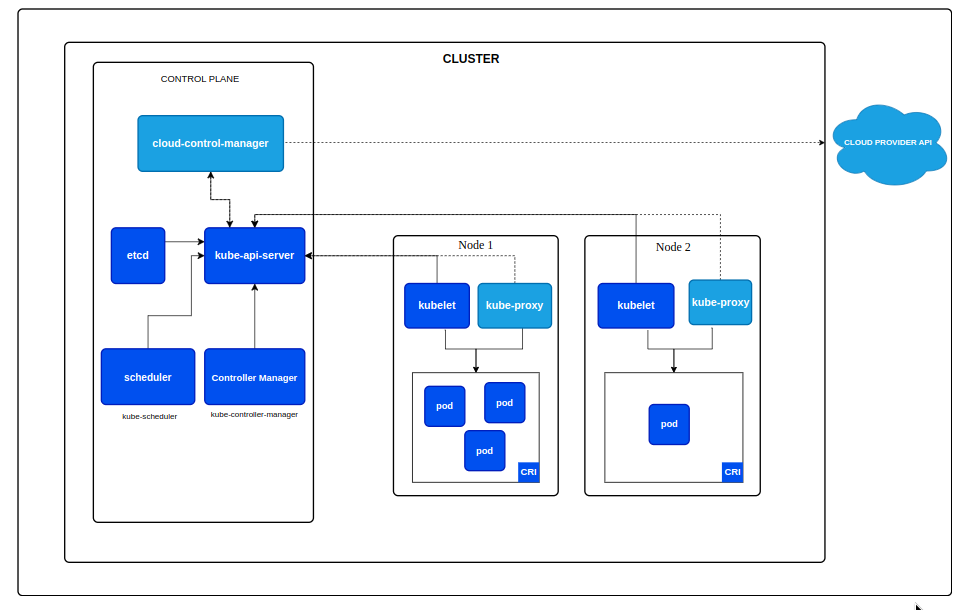
\includegraphics[width=0.8\textwidth]{assets/tools/kubernetes/kubernetes-architecture.png} % Change this to your image file
    \caption{Kubernetes Architecture: High view}
    \label{fig:sample-image} 
\end{figure}

Another concept worth mentioning is the distinction between \textbf{Pods} and \textbf{Containers}. \textbf{Containers}, like mentioned before, are lightweight boxes of software that include everything needed to run an application, offering \textbf{isolation}, \textbf{portability}, and \textbf{efficiency}. On the other hand, \textbf{pods} are the smallest unit deployable unit within the \textbf{kubernetes} logic and represent a logical host for one or more containers, which can be more or less as another box but just to put containers in it. It shares both storage and networking resources, being as well the fundamental building block for running applications and services.

\begin{figure}[H]
    \centering
    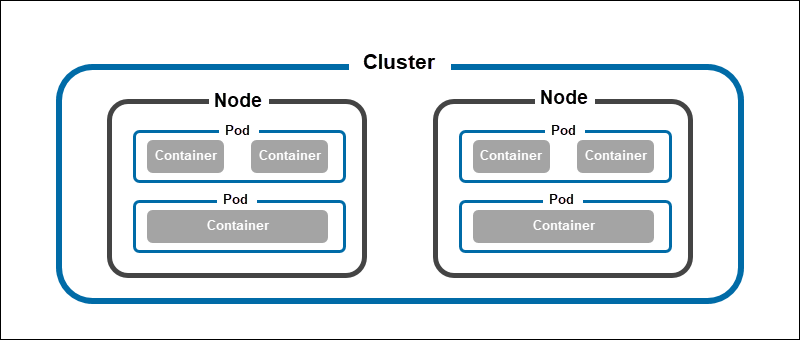
\includegraphics[width=0.8\textwidth]{assets/tools/kubernetes/pods.png} % Change this to your image file
    \caption{Representation of pods within a cluster}
    \label{fig:sample-image} 
\end{figure}

When it comes to \textbf{Microservices}, \textbf{scalability}  and \textbf{load balancing} have a notorious complexity and importance. This is elevated to a more extreme level when it is combined to \textbf{kubernetes}. \textbf{Scalability} refers to the capacity of increasing resources, where this increase could be done in two major ways: \textbf{Horizontal Scaling} and \textbf{Vertical Scaling}. \textbf{Horizontal Scaling} happens when there is increase or decrease of instances of the same application where by using a service can receive balanced traffic and thereby work together for the same goal, which in the case of \textbf{kubernetes} are \textbf{pods}. As an example, lets think of an web application in go, which serves a API to retrieve records of something. Within a given time-frame, there is a increase of demand such that a unique instance of this application is not enough. To make the service meet the demand, the operator increases the number of \textbf{replicas} of the same service "go-service". Because this service is targeting both instances (replicas) that are actually the same application, when a bunch of users request the records the traffic is spread among this 2 same instances making the server able to use more resources and serve more requests by having two instances. After the demand decreases, the operator can reduce the number of replicas and leave only 1 to save resources. \textbf{Vertical Scaling}, on another perspective, is a way that can also be used to meet increase or decrease of demand but more related to hardware. As an example lets say there is the same case described before but this time the application is incapable of serving well its users because it's CPU is already exceeding what he can do. With this practical, the operator can escalate vertically upwards to meet the demand by adding CPU and downwards to save resources in case the demand turns out to reduce once again \cite{vertical-scaling}\cite{horizontal-autoscaling}\cite{scaling-vertical-and-horizontal}. Within this scope it is important to mention that \textbf{Kubernetes} has mechanisms for making this scalation automatic by using metrics, which are \textbf{VPA}(Vertical Pod Autoscaler) and \textbf{HPA} (Horizontal Pod Autoscaler). \textbf{Load Balancing}, in another perspective is spreading the traffic among this multiple instances, making sure that none gets overwhelmed \cite{load-balancing}.

\textbf{Service Discovery} and \textbf{Networking} are important things to know when it comes to kubernetes. It's exceptional for making communication between various services and pods of the cluster where it's understanding it's important for deploying applications. The \textbf{Service Discovery} is a mechanism that allows applications and services to discover others inside the cluster. To make this possible, it requires methods such as \textbf{DNS-Based Service Discovery}, which allows pods to communicate with each other using its fully qualified name \textbf{(FQDN)}, such as \textbf{my-service.my-namespace.svc.cluster.local} and \textbf{Environment Variables}, which are injected in each service, making pods enabled to know the existence of others's by existing settled variables. \textbf{Networking}, on the other hand, is a model that abstracts the complex realm of the communication between containers, pods, and services. For reaching this abstraction, it uses 3 components such as \textbf{Pod Networking}, where each pod has it's own unique IP address and the containers within the pod can communicate with each other using \textbf{localhost}. Containers inside of a given pod can communicate with another container inside of another pod by levering their assigned IP's or by using the component \textbf{Service Networking}. \textbf{Service Networking} is a way that pods can use to abstract their access, either by using a gateway such as a load balancer or by using the service name within the cluster. Finally, there is a \textbf{Network Policies} component that can be used to define rules for ingress and egress traffic between pods. Ingress means the internal traffic, and egress is the external traffic. This is used to control how the internal and external traffic can flow inside of the cluster.

Configuration and secret yielding are a need for every microservice. Is it to retain keys for accessing an API, a password, or even a certificate? This is needed to make connections between a certain number of services while making sure that the services exchange messages with a given degree of security. With this in scope, \textbf{Kubernetes} offers configuration management and secrets out of the box. Thus, as responsible for this, there are \textbf{ConfigMaps} and \textbf{Secrets}, but both serve 2 different use cases. \textbf{Config Maps} are used to store non-sensitive configuration in key-value pairs like environment variables, configuration files, and even command-line arguments that can be passed at runtime to containers without the need to rebuild the containers, serving as an extension to the proper existing environment variables in the pod configuration but without the need of resetting the pod, being changeable at any time. As an example, there is the case where a given property may change in relation to the environment that is under target. A development environment may have its own database and staging another; therefore, there is the capability to change the connection configuration, making it feasible to change without having to restart everything but instead changing just the key value pair in this store. However, in the opposite direction, \textbf{Secrets} are deeply related to storing sensitive information, such as passwords, API keys, and certificates. It is stored in base64 format, and Kubernetes has its own mechanisms to securely save this. It is recommended that an organization that wishes to implement this carefully consider the existing security vulnerabilities \cite{config-management-and-secret}.

For achieving persistence storaging within \textbf{Kubernetes}, there are 2 major concepts that must be known. One is for creating volumes that a application may try to own further \textbf{PV's} (Persistent Volumes), and the other for making the actual request to own a given persistent volume \textbf{PVC's} (Persistent Volume Claims). \textbf{PV's} abstract the storage implementation that can be either local, using \textbf{NFS}(remote storage) \cite{nfs} or cloud-based, while still providing various access modes to that volume, such as \textbf{ReadWriteOnce}, \textbf{ReadOnlyMany}, and \textbf{ReadWriteMany}, which specify the type of permissions over it and how many pods can access it. As an example, \textbf{ReadWriteOnce} gives read and write privileges, but only one pod can actually mount it.

Like mentioned before, there are a certain group of components responsible for managing the smallest unit that a Kubernetes cluster can have (pods). This components can be used to watch the state of a cluster and make a set of actions to bring this state closer to the state that the user mentioned in it's configuration file, which means that they continuously monitor the cluster and work to make its state converge to the desired state. The existing types for a \textbf{kubernetes controller} are: \textbf{Deployment},\textbf{ReplicaSet},\textbf{StatefulSet},\textbf{DaemonSet},\textbf{Job and CronJob Controller},\textbf{ReplicaSet Controller} and \textbf{HorizontalPodAutoScaller}. As first, \textbf{Deployment} is the most used type of controller. It is widely used to deploy and manage stateless applications, making sure that they have high availability and controlled rolling updates. This is done by making sure that a desired number of replicas is maintained for a specific application and that these replicas are running all the time, which usually implies automatically handling scaling, updates, and rollbacks. In second, \textbf{ReplicaSet} is what the \textbf{Deployment} manages to maintain the replicas, and it is used to ensure that these replicas keep running. \textbf{StatefulSet}, on the other hand, is another useful controller that shares characteristics with the deployment, but the difference relies on the type of management required, which according to the nature of the pods in question is different. \textbf{Deployment} is for stateless applications, while \textbf{Statefulset} is for "Stateful". What this means is that the \textbf{deployment} deletes random pods in a scale down and adds pods with random identifiers while the other adds and removes pods sequentially, which helps in certain situations in pods with states. As an example, there are databases that are distributed that are based on a consensus algorithm. To scale down those effectively, there is the need to scale nodes sequentially and not in parallel like in deployments, making the removal and addition of nodes more constant; thereby, in case nodes are removed, the consensus algorithm will not be unstable and the service will remain available despite this removal. \textbf{DaemonSet}, on the other hand, is a pod that is obligated to run per node within a cluster, making it feasible for logging, monitoring, and network cases that require an instance per node. As an example, there is cadvisor that requires an instance per node for collecting data for metrics. For temporary pods, there is also the \textbf{Job and CronJob}, which runs pods that are designed just to fill temporary tasks such as backups and data processing. Finally, \textbf{HorizontalPodAutoscaler}, however, is a controller that manages the horizontal scaling by looking into metrics such as CPU utilization, memory usage, or custom metrics.

Security within the \textbf{Kubernetes} cluster remains one of the major concerns in the industry. This is because of its complexity and widespread adoption, making it a must in organizations, and at the same time, because of its complexity, something that could be targeted from anywhere within its scope. The proof of this is that security for this technology continues to be the most debated topic, promising 12.3\% of overall topics, which means that securing this technology is a priority among users in the \textbf{kubernetes} sphere \cite{kubernetes-security-concerns-yet}. However, there is also some work related to the analysis done around security reports oriented to \textbf{kubernetes}. More concretly, according to some works, security breaches in kubernetes are extremely underreported, with 0.79\% commits related to security. This reveals that further research must be done to actually spot hidden security vulnerabilities, thereby strengthening security practices \cite{under-reported-kubernetes}. Also, there is an increase in the usage of AI for anomaly detection, which has been showing improvements in threat detection... spot more 92\% and reduce response times by 67\% compared to traditional methods \cite{ai-k8-spot}. Nevertheless, there are also assumptions chattered by Helm charts, evidencing that half of the container images used are outdated and 88.1\% of those images are exposed to vulnerabilities \cite{helm-images-vulnerabilities}.

Relatively to the importance of this tool for this thesis, it should be known that the intention is not to simply create a blockchain application but instead gather the best that the market has to offer and create seamlessly coordination between web2 and web3 technologies. With this in mind, all of the use cases displayed here make use of such, taking advantage of all of the best capabilities that kubernetes can offer for such a big organization as a healthcare one.

\paragraph{3.5.2.2- Docker}\mbox{}\\
\textbf{Docker}, on the other hand, is a  technology that could be abstracted by the previously mentioned \textbf{Kubernetes} and is said to be a tool to build applications in a different paradigm than before. To contextualize, in the past it was something normal to install dependencies directly in your local machine, which created some burden since you may have had different projects with different dependencies versions. Also, the application would mess with the local machine configurations because it was directly using it's resources, having more probability of making adjustments that would compromise other projects by having different configurations. By acknowledging these limitations, Docker came to light because it was conceded to automate deployment, scaling, and management of these referenced applications using a new concept called \textbf{containerization}. 

Before containers, there was a concept called \textbf{virtualization}. This is still widely used, but it became less with the introduction of containers. This is because, despite being very powerful, \textbf{virtualization} is more heavy than a container, though offering the same characteristics.

The main advantages, on the other hand, for this tool are \textbf{isolation} from the operative system, the possibility to run \textbf{more instances} compared to VM's, \textbf{portability}, \textbf{more collaboration} within the team, \textbf{version control}, \textbf{streamline process} capability, and the capability of \textbf{scaling} if used along side kubernetes. Thereby, it's main features are: \textbf{Lightweight Virtualization}, \textbf{Containerization}, \textbf{Portability}, \textbf{Isolation}, \textbf{Version Control and Reusability}, and \textbf{Scalability and Efficiency}.

Due to its importance not only within this project but also the current landscape of technology, it is considered a very special tool; therefore, it will be discussed here in this section.

\textbf{Containerization},like mentioned before is a technology in software engineering to package all dependencies and software all together, creating a environment that shares the kernel with the host but isolates the rest of the resources, while being a lot more light than VM's. Because of this,the application runs in any kind of environment, since this creates isolation. By the cause of such, the main characteristics associated with \textbf{docker} are \textbf{Isolation}, since processes,memory and file systems are totally segregated, such that multiple containers can run without interference with each other. \textbf{Portability}, because it packages everything in a single unit. \textbf{Efficiency}, due to the fact that is very lightweight and \textbf{Scalability} because it can be scaled up or down easily and there are orchestration tools that make this even more easier such as the previous mentioned \textbf{Kubernetes}.

To understand how Docker works, there is the necessity to view how it's architecture is composed. With this in mind, the main core components of Docker are the following: \textbf{Docker Client},\textbf{Docker Daemon(dockerd)},\textbf{Docker Images},\textbf{Docker containers},\textbf{Docker Registry}, \textbf{Docker Network} and \textbf{Docker Volume}. \textbf{Docker Client} is responsible for sending requests to a given instance of the Docker daemon. This instance can either be locally or remotely located in another machine. To make such communication there are commands such as \textbf{docker build}, \textbf{docker run} and \textbf{docker pull}. \textbf{Docker Daemon(dockerd)} is the one that is responsible for managing containers on the host system while ensuring isolation and resource management between containers. Also, this is also what is responsible for serving requests from the Docker client, making it able to manage Docker objects like containers, images, networks and volumes. \textbf{Docker Images}, on the other hand, are read-only templates that define the structure that a container should have. This template contains everything related to an application, like code, runtime, libraries,environment variables, and configuration files, and is usually created accordingly to a \textbf{Dockerfile}, where it gathers all the necessary instructions for setting up an image. \textbf{Docker Containers} are instances that could run that came from a previously created template (Docker image). Each instance can run without affecting others', but it does share resources over the machine they are running on. They have their own file system, network and process space. \textbf{Docker Registry} is another important component, which is where images can be published. This publication is done in a remote repository that can be later used to download and use images as intended in our applications. This registry can either be public or private, giving power to those who use it. \textbf{Docker Network} is what enables the communication between containers. This container can be either on the same host or across multiple hosts, having several networking drivers like \textbf{bridge}, \textbf{host}, and \textbf{overlay}. Finally, \textbf{Docker Volume} is the persistent storage that a container can have. This is done by mapping the container file-system with the host, which otherwise would be always resetting every time a new container is created, which may not be feasible in some situations.
\begin{figure}[H]
    \centering
    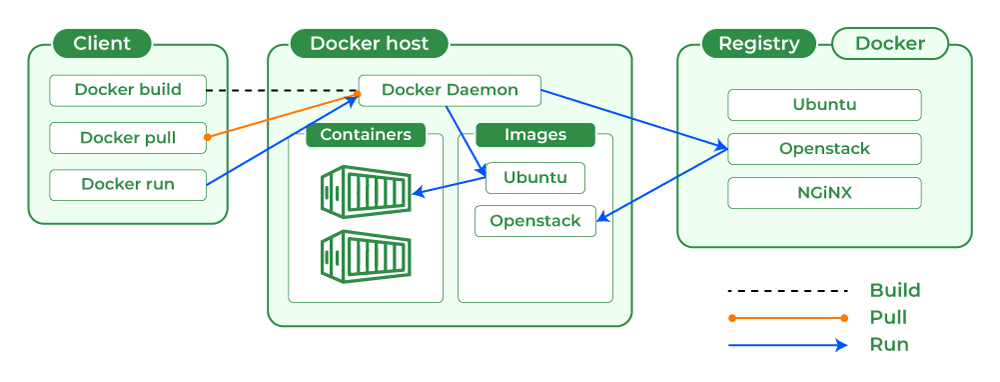
\includegraphics[width=0.8\textwidth]{assets/tools/docker/Architecture-of-Docker.png} % Change this to your image file
    \caption{Docker architecture: simple view}
    \label{fig:sample-image} 
\end{figure}

In the realm of the \textbf{docker security}, it has a lot of features that contribute for this to be ensured. However, there must be configured accordinally, otherwise it may not be as much effective as it should. With this covered, there are several features that docker disposes that actually help establishing this type of securance like \textbf{Namespace Isolation},\textbf{Control Groups(cgroups)},\textbf{Read-only file systems},\textbf{user namespace},\textbf{security capabilities},\textbf{Seccomp},\textbf{AppArmor and SELinux} and \textbf{Image Security}. \textbf{Namespace Isolation}, is a method to isolate even more containers and the host system by sogregating its network,users and mounts. \textbf{Control Groups}(cgroups) are groups used to limit and prioritize resources such as CPU,memory and disk I/O among containers, which prevent containers of consuming resources excessively. \textbf{Read-only file systems}, is another feature which enables the container of being only allowed to read and not modify it's file system. With this malicious actors cannot modify or inject malicious code during the runtime. \textbf{User Namespaces} is responsible for running containers as non-root users, making unfeasible the possibility of malicious actors to scalate it's privileges to another containers, therefore only comprimising a single container. \textbf{Security capabilities} are a set of capabilities that the administrator can set for a container to be dotted of. By default this containers already come with a certain number of capabilities that are not harmful. However, the administrator should understand and add or remove them accordingly to it's need to make sure that the application remains the most secure it can be. \textbf{Seccomp (Secure computing Mode)} however, its another feature which is composed by profiles that reduce the number of systemcalls that a container can do. This systemcalls are calls that are made directly to the hardware and if profiles are well settled, a good defense against potential exploits is present. \textbf{AppArmor and SELinux} are security modules to enforce access control policies, providing mandatory access control on the host system. This ensures that containers can only use resources defined by this policies. Finally, there is \textbf{Image Security}, where docker offers a command for scan a image in order to detect it's vulnerabilities. This command is \textbf{docker scan}. Also, there are plenty of information regarding good practises in docker such as \textbf{Use Official and Trusted Images},\textbf{Least Privilege Principle},\textbf{Enable Read-Only File Systems},\textbf{Limit Network Access and Inter-Container Communication},\textbf{Regular Vulnerability Scanning},\textbf{Usage of Docker Content Trust (DCT)},\textbf{Implementation of Seccomp,AppArmor or SELinux Policies} and \textbf{Avoid Storing Secrets in Images} as an example \cite{docker-good-practises1} \cite{docker-good-practises-2} \cite{docker-good-practises-3} \cite{docker-good-practises-4}.

This tool is core for \textbf{CI/CD Pipelines}. \textbf{Continuous Integration} (CI) is a pipeline that aims to create a flow for code, build, and test applications, while \textbf{Continuous Development} (CD) is a pipeline for release, deploy, operate and monitor applications. To achieve this, \textbf{docker} is the tool that is used to build images, to release, deploy, and to monitor. These practices are very important because they speed up the development, thereby making Docker very important from this perspective. Also, another usage of Docker is within the \textbf{kubernetes} realm, since this is the containerization technology that is often more used. Kubernetes requires Docker because it manages containers, where Docker fits religiously.

Also, docker is very important in this thesis since it has all of the characteristics covered so far and it's used across all of the use cases.

\paragraph{3.5.2.3-MetalLB}\mbox{}\\
\textbf{On-premise cluster} is an advanced concept related to setting a network of computers within your own infrastructure. In the case of this project, the reference to this is related to a network composed of \textbf{kubernetes} nodes. Because of this, it is imperative to mention \textbf{MetalLB}, which is a \textbf{load balancer} conceded just for \textbf{on premise Kubernetes clusters}.

When it comes to \textbf{kubernetes}, usually the tendency is to relate it to the cloud. However, as the time progresses, components become more powerful and cheaper, and more and more, the consideration of moving to the cloud or not becomes more a question of cost and responsibility. This is because, though the power of components is becoming stronger, the complexity of hardware is sometimes increased, making organizations choose between being themselves responsible for the maintainability of the infrastructure or simply giving it away to those that are more specialized in the subject, which may or may not reduce costs for them because not only do they have the common infrastructure costs but also the burden of finding and maintaining qualified personnel for this type of job \cite{onpremice-cloud}.

\textbf{MetalLB} comes into play when it comes to those more audacious to have all the responsibility. As a strong \textbf{Load Balancer} for \textbf{on premise} networks, it stands in this project as a marvelous tool. 
for achieving load balancing, which is a concept where the requests are distributed through multiple instances of the same application, balancing this way the load that each may have. Cloud distributors have their built-in support for such, while on-premise networks do not, which makes \textbf{MetalLB} a must for setting such capability in a non-cloud environment.

With this in mind, with features such as \textbf{Load Balancing for Bare-Metal Kubernetes}, \textbf{Layer 2 and Layer 3 Modes (BGP Mode)}, \textbf{Address Pool Management}, \textbf{Seamless Integration with Kubernetes}, and \textbf{High Availability}, \textbf{Metalb} is indeed a genesis block when it comes to mirror cloud environments locally, therefore this section will be covering it at its best.

To put it more clearly, the need for \textbf{MetalLB} in Bare-Metal Kubernetes cluster has to do with several reasons, such as: \textbf{Lack of Cloud Load Balancer Services}, \textbf{Direct Integration with Bare-Metal Network Infrastructure}, \textbf{Ease of Configuration and Flexibility}, \textbf{Avoiding the Need for External Hardware Load Balancers}, \textbf{Support for LoadBalancer Type Services}, and \textbf{Scalability and High Availability}. In regards to the \textbf{Lack of Cloud Load Balancer Services}, this means that on-premise there is no load balancer out of the box like in a cloud environment. Thus, in the cloud there is no need at all to implement your own, while in your own infrastructure there must be a settled one; otherwise, load balancing will be a feature out of scope. Direct Integration with \textbf{Bare-Metal Network Infrastructure} means that \textbf{MetalLB} can integrate this functionally directly with the existing infrastructure. This is done either with IP advertising in \textbf{Layer 2 mode (ARP)} or with \textbf{Layer 3 (BGP) mode}. \textbf{Ease of Configuration and Flexibility} because \textbf{metallb} it's easy and flexible to configure, like it will be mentioned in future use cases. \textbf{Avoiding the need for external hardware load balancers} it's also another good characteristic, which means that, while other organizations resort to the usage of expensive hardware for load balancing or complex software-defined networking, \textbf{Metallb} offers a software-based and yet native approach to manage the necessary operations to come up with this load balancing \cite{hardware-vs-on-premise}. \textbf{Support of LoadBalancer type services} is another big factor, since without a load balancer this is not possible, where \textbf{metallb} comes into action. Finally, \textbf{Scalability and High Availability}, since it can scale with the number of nodes within the cluster, distributing service traffic evenly across multiple nodes.

Speaking about it's architecture, it should be known that it's simple but yet powerful. It has a brain by the name of \textbf{controller} that monitors the Kubernetes API server for services that require a load balancer, thereby deciding how to allocate IP addresses on them, while still being responsible for managing the state for each of the load balancer services, ensuring that the right configurations are established for further well-conducted external connectivity. At it's core, it also has the \textbf{speaker}, which is a component that announces the external IP's using protocols such as \textbf{Layer 2} or \textbf{Layer 3}, enabling this way the cluster to communicate with the external network, making services accessible outside the cluster. As a finishing term, there is also the already mentioned protocol, which is the \textbf{Layer 2} mode, where the speakers announce the IP's by levering l2 capabilities such as the \textbf{ARP} \cite{arp} protocol within the local network segment. This mode is more suitable for smaller clusters, where the \textbf{L3} is more suitable for bigger clusters. This is because l3 uses a \textbf{Border Gateway Protocol}(BGP) \cite{bgp} \cite{bgp2} that advertises the IP addresses to external routers while also offering advanced capabilities such as networking policies and fault tolerance.

Within a more deeper analysis of \textbf{l2} mode, it must be known that it works under a local area network (LAN). This is the simpler configuration mode supported by \textbf{metalLB} and works with the leverage of both \textbf{ARP} and \textbf{NDP} to advertise the presence of a service IP within the local network. With this implementation, what happens is that a ip address is generated from a pre-defined pool of ip addresses and then, recurring to ARP, it announces a given IP that then is requested to the network and exchanged by a \textbf{MAC} address.

On regards to \textbf{l3}, on the other hand, it works using external routers. This makes it more suitable for larger clusters or envronments where complex routing and multi-subnet configurations are required. Also, it offers more advanced capabilities such as network policies and fault tolerance. It works by making sure that a given external router is compatible with the speakers, it communicates with them to check the ips to be advertising and makes those available outside of the cluster where any request will pass throught them and get redirect to the correct node in question.

\begin{figure}[H]
    \centering
    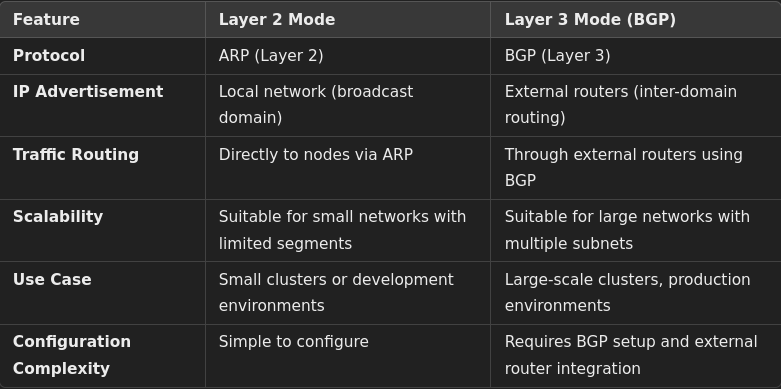
\includegraphics[width=0.8\textwidth]{assets/tools/metallb/bgp-vs-l2.png} % Change this to your image file
    \caption{Layer 2 vs Layer 3 Mode}
    \label{fig:sample-image} 
\end{figure}


To use this extension, it must be known which kind of \textbf{Kubernetes} service can be used to expose the traffic. In the case of \textbf{MetalLB}, the only service that he does support is the \textbf{LoadBalancer} type. However, there are a lot of others that may be discussed forward.

Within a lot of major capabilities, \textbf{MetalLB} also offers both high availability and failover. Such ensures that services remain accessible even in the case of node failures or network problems. High availability is achieved with both \textbf{L2} and \textbf{L3} modes, depending on the network configuration and it's specific requirements. As an example, when a failure occurs in a L2 implementation and one of them goes down, it rapidly selects another node for that precise IP, while in a L3 mode, there can be implemented an equal-cost multi-path routing, which allows multiple nodes to advertise the same IP and switch the IP to another node in case this node goes down.

The importance of such in this project is that most of the healthcare system's relies on an on-premise network. Doted of such, and in case there is a Kubernetes network, it is very important to have a mechanism to create load balancing for some precise components, which will be occurring within the use cases realm.

\paragraph{3.5.2.4- Istio}\mbox{}\\
In this thesis, \textbf{Istio} appears more like an extension and not concretely as something that was of extreme usage. However, because it was used to determine whether each measure is useful and also because it is very different from other concepts, explanations over what it is are required because, although not extensively used, it is mentioned in the thesis.

\textbf{Microservices} is an architecture of exalted power. However, what comes with great power also requires great responsibility. Therefore, conducting the management of the communications between services is not a straightforward task. By virtue of such, the more the application expands, the more work there is around this matter, making \textbf{DevOps} teams struggle when it comes to make optimization and manage this within the application realm.

By means of this, \textbf{Istio} surges as alleviation of such. At the hand of its capabilities, it serves as a \textbf{service mesh}, which is nothing more than an abstraction created around the application for providing \textbf{Traffic Management}, \textbf{security}, \textbf{Load Balancing}, and \textbf{monitoring}.

As mentioned before, cloud-native architectures and microservices are becoming something permanent. Such that managing it is a challenge. Thus, using a \textbf{Service mesh} could potential be something meaningful because it works as an abstraction layer that handles the dynamic networking and communication between microservices. With this brief introduction in mind, thinking in the most important aspects for which this is needed is something intriguing. Firstly, \textbf{enhances microservice communication and networking} is one of the aspects for including istio. This is because, a service mesh provides service-centric networking, thereby oferring features that are not native to kubernetes. This is helpful for managing services communications with capabilities such as load balancing,retries,timeouts and circuit breaking \cite{service-mesh-enhance-communications}. In second, despite current implementations create overhead in terms of resources, due to the proxys and the new side containers, there are service mesh implementations that actually aim to \textbf{improve performance and resource efficiency}. This can be done with new architectures like \textbf{FlatProxy}, which reduce performance bottlenecks and improve resource utilization \cite{service-mesh-flat-proxy}. As a third motive, there is the aspect of \textbf{Observability and Monitoring}. This as to do with the fact that a service mesh collects metrics,traces and logs for each service interaction, providing insights about the behavior of the microservices enabling performance bottlenecks spotting, understading of service dependencies and improving system debugging \cite{service-mesh-monitoring}. In forth, it should be known that it also facilitates traffic management through fine-grained control policies, such as traffic splitting,canary releases and fail-over strategies. However, there are studies affirming that it creates overheads such as 269\% latency and 163\% CPU usage, emphasizing the need for optimization \cite{service-mesh-traffic}. When it comes to the final, the \textbf{Security and Resilience} is another aspect that serves as a benefit to use it since a service mesh usually offers mutual tls out of the box with certificate rotation \cite{service-mesh-security}. 

When it comes to the \textbf{Istio Architecture}, there are two major main components such as \textbf{Control Plane} and \textbf{Data Plane}. The \textbf{data plane} handles all the network traffic between services. This is furnished using \textbf{Envoy proxies}, which is a sidecar container or a container that stands in addition to the main container. This side container catches and controls all inbound and outbound traffic for the service. With such an broker, the given service gains extended network capabilities like load balancing, enforcing policies, collecting telemetry, routing, and observability. The \textbf{control plane}, on the other hand, manages and configures the proxies from the data plane. It had several valuable components, such as \textbf{Pilot}, \textbf{Citadel}, \textbf{Galley}, and \textbf{Istiod(Unified Control Plane)}. The \textbf{Pilot} is the component that is responsible for service discovery, traffic management, and distribution to envoy proxies that translate high-level routing rules into configurations understood by envoy and push them to the proxies. The \textbf{Citadel} manages all the security mechanisms, like the security in the communications and certificate distribution, providing strong service identity and mutual TLS communication between services, and automating key and certificate management for service-to-service authentication. \textbf{Galley} validates and processes configuration files before distributing them to other components, while ensuring that only valid configurations are applied, reducing this way the errors. Finally, \textbf{Istiod(Unified Control Plane)} is the aggregation of Pilot, Citadel, and Galley in the new versions.

In the sphere of \textbf{traffic management}, more concretely, referring to the \textbf{Istio} landscape. This is an existing concept for enabling fine-grained control over the flow of traffic among services by leveraging routing rules, controlling the flow of traffic, and implementing fail-over policies to ensure reliability and robustness. To make this happen, there are several resources that can be used within the configurations that could be used to manage such, like \textbf{Virtual Services}, \textbf{Destination Rules}, \textbf{Gateways}, and \textbf{Sidecars}. \textbf{Virtual Service} defines how requests are routed to a service within the mesh by setting rules that could describe how requests should be forwarded based on characteristics like path, HTTP headers, or traffic weight distribution. \textbf{Destination Rule} are the rules destinated to a specific service or a subset of a service, like load balancing settings,connection pool sizes, and outlier detection. \textbf{Gateway} configures how traffic enters and leaves the service mesh, enabling to specify the behavior in ingress (incoming) and egress (outgoing) traffic. \textbf{Service Entry} is to manage outbound traffic to services that are not apart of the mesh, and \textbf{Sidecars} configures the sidecar proxy behavior for a specific workload.

\textbf{Security} measures for such helpers in traffic management are another thing to take into account. To conquer this, Istio offers features for authenticate, authorize, encrypt and provide identity management. This is helpful because it removes the need for the operator to implement such things in the application itself, thereby segregating the application security from the application and making it easier to change settings as time proceeds. It provides \textbf{Authentication} by ensuring the identity of both services and users is valid. This is achieved because it has mutual TLS with automatic rotation for both clients and services, while also offering JSON Web Tokens (JWT) for end-user authentication. It provides \textbf{Authorization} because it has \textbf{AuthorizationPolicies} that define what kind of actions are actual permitted or denied based on attributes such as source, destination, and content requested, while allowing to apply them at the namespace, workload, and service level. It also lets us change the \textbf{mutual tls} behavior, mentioning if there can be a hybrid approach of both mtls and plaintext traffic or if this mtls should be strict to the point that only mTLS traffic is accepted. \textbf{Identity Management and Certificates} is also offered by creating a unique identity in the form of a \textbf{SPIFFE}(Secure Production Identity Framework for Everyone) URI, which is tied to the service account in Kubernetes. Offers \textbf{Security policies} for defining authentication settings like \textbf{PeerAuthentication} and \textbf{RequestAuthentication} and for authorization settings such as \textbf{AuthorizationPolicy}. Finally, it also offers security among \textbf{ingress} and \textbf{egress} traffic, which also molds the behavior of the traffic that enters or gets out of the cluster.

Since this works out of the box like an abstraction over the traffic, it becomes clear that observability and monitoring over it would be feasible. What can be found here is \textbf{Metrics collection} , \textbf{distributed tracing} , \textbf{logging} , and \textbf{visualization capabilities} . Relatively to \textbf{Metrics collection} , they cover an amplified range of matters, covering HTTP and TCP traffic. This data is usually in time-series format, where Prometheus comes to play to be its widely used collector. This way, Prometheus usually collects the data, and Grafana presents it to someone. Some of the metrics that can be found are something like \textbf{istio\_requests\_total} for the total number of requests that a service received,\textbf{istio\_request\_duration\_seconds} for measuring latency in seconds, \textbf{istio\_request\_size} for checking the size of the requests received,\textbf{istio\_response\_size} for checking the size of the requests sent and \textbf{istio\_tcp\_connection\_opened\_total} for the total number of TCP connections opened. For \textbf{distributed tracing} , there are integrations with tracing tools such as \textbf{Jaeger} , \textbf{Zipkin} , and \textbf{OpenTelemetry} , which allow us to understand the existing flow of communications between services, helping in debugging, bottlenecks, and error detection. Also, within the \textbf{logging} realm, Istio offers a generation of logs for all the service requests and responses, providing detailed information about such, which is imperative for things like troubleshoot detection, auditing of service interactions, and paths and headers monitoring. For visualization capabilities, on the other hand, Istio also offers good options, such as the integration with \textbf{grafana} and \textbf{kiali} . For both, existing dashboards are already at the disposition of everyone, which means that little configuration must be done, though Grafana is more suited for all and Kali is more custom-made to service meshes, presenting more capabilities out of the box.


\textbf{Service Discovery} and \textbf{load balancing} are key components from Istio. The first helps services discover each other, and the second one balances the traffic efficiently within the mesh. This is important because in microservices environments the number of components is not always constant; thereby, there must be some kind of mechanism to make their increase or decrease automatic with little configuration involved. Relatively to the discovery, Istio first retrieves information about services and their associated endpoints. Secondly, all of the services and endpoints are stored in a specific service registry, maintaining this way up-to-date information about service endpoints, IP addresses, and port mappings. Thirdly, the service discovery information and traffic management rules are pushed to the envoy sidecars, enabling sidecars to perform with the most recent service state. Forthly, the sidecars use the service registry information to make intelligent routing decisions, like selecting the appropriate instance of a service based on the available endpoints and configured load balancing strategies. Finally, by the usage of the previous spoken \textbf{ServiceEntry}, the Istio adds other external services to it's registry, enabling them to be there like they are apart of the mesh. In the behavior of the load balancing, on the other hand, it gets configured by \textbf{DestinationRule} resources. Also, it has a lot of different strategies such as \textbf{Round Robin} which is a default and simply distributed its traffic evenly, \textbf{Random} which randomly selects a service to handle the request, \textbf{Weighted Least Request} which routes the traffic to the instance with the least number of active requests, \textbf{Ring Hash} which maps requests using hashes, \textbf{Consistent Hashing} which behavior is alike \textbf{Ring Hash} but for managing the requests from a given client to a concrete backend, \textbf{Least Connection} to redirect to the instance with fewer active connections, and \textbf{Passthrough} which forwards the traffic to the backend without any load balancing.

The key component of Istio is the sidecar container based on \textbf{envoy}. This is what is deployed along with each service within the mesh, offering security, traffic management, observability, and resilience for microservices while ensuring compliance with policies, traffic splitting, security enforcement, and telemetry collection. It is a high-performance edge and service proxy designed for cloud-native applications and has become the default data plane for Istio.

Istio is also doted with multiple features to increase reliability. These features are very well known in the distributed systems context and tend to help ensure that microservices can handle graceful failures, prevent cascading issues, and provide robustness in complex service interactions. These services are: \textbf{Circuit Breaking}, which is a pattern used to prevent a system from repeatedly making requests to the same failing system. When a given number of requests fail, this mechanism blocks the service for a given period of time, enabling him to recover and avoid it's exhaustion; \textbf{Retries} are another mechanism, but it stands for retrying the request in case it fails before returning an error to the client, and \textbf{timeouts} for a maximum time that a service should wait for a response from another service. In case the request exceeds this timeout, the request gets terminated \cite{circuit-break-and-timeouts}\cite{circuit-breaking-and-retries-2}\cite{circuit-breaks-and-retries}.

Finally, the last capability of istio is something related to it's flexibility. With istio there is the possibility to create single to multi cluster deployments and single to multi network models as well, making is feasible even for segregated environments.


\subsubsection{Analytics}
This chapter centers it's focus in Analysis. When there are ideas about a given system, usually people don't think right ahead on this matters. Despite the possibility of creating systems without such capabilities, it will become clear further in time that it will be painful and more like a burden if there are none, this is because, the more complex the system gets the more there is a need to auditing and this is only possible if there are mechanisms prepared for the analysis of the network. In other words, despite not directly mandatory, it is almost a obligation to make our infrastructure doted of such, because by having good design over the analysis, auditing becomes more easier and there is the possibility of knowing where to do better by spotting, for example, bottlenecks but also where in the system something is failing (debug). Also, there is a need of having tools that simulate real behavior from users so that the responsible knows the limits of the given System. With this in mind, in this section, it will be covered all of the tools that in conjunction are used to deliver this capabilities that were just spoken. Firstly there will be a discussion about \textbf{Caliper} which is a framework to benchmarking blockchain networks, such as \textbf{hyperledger fabric} in our research projects. Secondly, there is \textbf{prometheus} overview which is a time-series data supplier. Thirdly, there will be information about \textbf{cAdvisor} which retrieves measures from machines and finally there will be a quick representation of \textbf{grafana}, because altought not used in the final implementation, it remains crucial for benchmarking since it has more visualisation capabilities for result comparison, which makes it more feasible than the ones built inside of the project.

\paragraph{3.5.3.1- Caliper}\mbox{}\\
In what respects the domain of \textbf{Benchmarking}. It is well familiar that it represents the \textbf{measuring} and \textbf{comparing of performance}. As the need of metrics arises during a project, there will be space for such concept and within this thesis this could not be different.

In prospect of the usage of such concept, within this project,there will be justification of results. Thereby, the need to use a tool such as \textbf{Caliper} and the requirement for further clarification of it, which will be stated in this category.

\textbf{Caliper} \cite{HyperledgerCaliper} is a open-source multi-function benchmarking tool. It is part of the hyperledger project and allows it's clients to evaluate various aspects of their blockchain implementations. This aspects could be \textbf{transaction throughput},\textbf{transaction latency},\textbf{resource utilization} and even \textbf{scalability}. Thought it's modular architecture, it is possible to implement a vast number of custom connectors, enable the developer to connect in various ways to multiple blockchains. Also, there is by standard connectors for a lot of network tastes such as \textbf{Hyperledger Fabric},\textbf{Ethereum},\textbf{Hyperledger Besu} \cite{HyperledgerBesu} and \textbf{FISCO BCOS} \cite{FISCOBCOS}. This flexbility allows those that have power over it to compare different solutions. Key features of it are: \textbf{Benchmarking Across Multiple Blockchain Platforms},\textbf{Customizable Performance Tests},\textbf{Detailed Performance Metrics},\textbf{Modular and Extensible Architecture},\textbf{Automated Benchmarking} and \textbf{Visualization and Reporting}.

Relatively to the key metrics in the hyperledger caliper, there is the \textbf{Throughput}, which is a measure of how many transactions a network can handle per unit time. \textbf{TPS (Transactions per second)}. \textbf{Latency}, which is the time taken for a transaction to be confirmed and added to the ledger after submission, \textbf{sucess rate}, representing the percentage of submitted transactions that were included, \textbf{transaction response time} is the time that a response takes to come from the network, including both validation and commit phases. \textbf{resource utilization} for measuring the usage of CPU, memory, disk I/O, and network usage across different nodes, \textbf{read/write operations} to measure the number of read and write operations performed during the execution of transactions; \textbf{commit time} to the time required for a transaction to be committed to the ledger after being validated; \textbf{block creation time} for the time it takes to create a block from validated transactions; \textbf{transaction ordering time} to measure the time taken to order transactions before they are batched into a block; and \textbf{failure analysis} to analyze the reasons for transaction failures like invalid input, lack of consensus, or even resource constraints.

Entering into the architecture of caliper, there are several concepts that could be spotted here. This key components are \textbf{benchmark module}, \textbf{adapter layer}, \textbf{monitor module}, \textbf{workload module}, \textbf{client and peer nodes}, and \textbf{reporting module}. The \textbf{Benchmark module} defines the overall testing workflow, being responsible for reading the user-defined benchmark configuration files, specifying workload settings, test duration, and the blockchain network to target. The file to configure all of this typically is the \textbf{benchmark.yaml}, including information such as the number of test rounds, transaction rate, and concurrency level. In the \textbf{adapter layer}, there is the abstraction of the communication with blockchain platforms, where each blockchain has it's own connector, and also there is the ability to create a custom-made connector as well, making it feasible to adjust things to the needs and even add new blockchains to benchmark. There is also the \textbf{Monitor module}, which tracks the system resource utilization during the benchmark test, capturing data such as CPU usage, memory consumption, disk I/0, and network activity, while also being able to integrate with Prometheus and Docker to collect these statistics, making the operator enabled to know performance analysis and bottleneck identification. \textbf{Workload module} is another component that is responsible for actually making sure that the workload state specified by the user is actually filled to come up with the scenarios. In other words, it's what controls rates and the number of transactions. \textbf{Client} on the other hand is what actually sends out the transactions to target the blockchain network peer nodes, such that they operate in parallel, simulating a realistic multi-client environment to stress-test the network. Finally, there is the \textbf{Reporting module}, responsible for aggregating the results for further analysis from the user side. It can generate these reports in various formats, such as JSON, HTML, and CSV. This report includes metrics like throughput, latency, success rate, and resource utilization.

\begin{figure}[H]
    \centering
    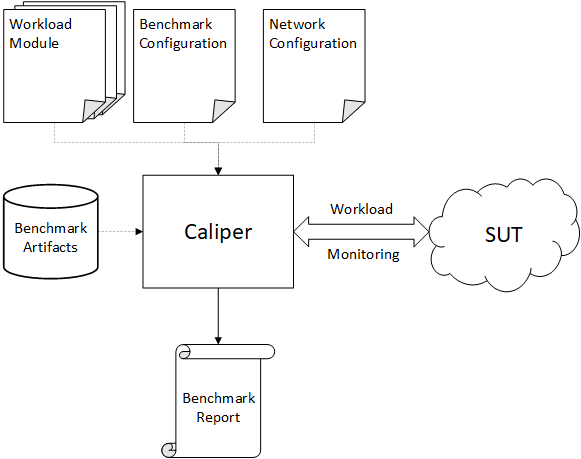
\includegraphics[width=0.8\textwidth]{assets/tools/caliper/arch_high_level.png} % Change this to your image file
    \caption{Caliper architecture}
    \label{fig:sample-image} 
\end{figure}

In order to come up with a benchmark, there are several workflow steps to be taken. Firstly, it should be defined as a benchmark configuration within the \textbf{benchmark.yaml} file, which includes network configurations, test scenarios, and workload parameters. Secondly, create the necessary configurations in the \textbf{network.yaml} and test it to see if it does work against the desired network. Thirdly, execute the workload module, which is the transactions that could be either of read type or write type. Fourthly, submit the transactions using the fabric adapter, connecting to the more suited node to ensure that transactions are validated, ordered, and committed to the ledger. Fifthly, the transactions get submitted and go through a validation phase where endorsement policies are checked. In case everything goes well, the transactions will be batched into blocks by the orderer and distributed among all the peers, giving a positive or negative response depending on whether it was successful or a failure. Sixth, the monitor module collects all of this data on system resource utilization, such as CPU, memory, disk I/O, and network usage in all participating nodes. Sept., there will be the reporting generation that the user must analyze. Finally, there is a result aggregation, and a final report is generated, which can be later used to take action over possible bottlenecks or misconfigurations.

\paragraph{3.5.3.2- Prometheus}\mbox{}\\
\textbf{Prometheus} is an open-source \textbf{monitoring} and \textbf{alerting tool} designed for recording real-time metrics. At the essence of this thesis, there will be instances where \textbf{Prometheus} is mentioned. This is because it is very useful to gather data from various places at the same time, making it easier to grab the data at a single point of failure. In other terms, it is a tool based on \textbf{time-series} and it remounts to the collection of metrics from various systems and services, making it very suited for this kind of project. Also, it provides various useful features such as \textbf{Time-Series Data Model},\textbf{Pull-based model},\textbf{PromQL},\textbf{Alerting},\textbf{Service Discovery},\textbf{Multi-Dimensional Data},\textbf{Efficient Storage} and \textbf{Dashboards and Visualization}.

More information about \textbf{Prometheus} will be delved into deeper in this category.

When crossing the architecture of Prometheus, it must be known that it has a lot of components in it, making it robust but at the same time reliable for aggregating sources of data. The key components of Prometheus are: \textbf{prometheus server}, \textbf{data storage and time-series database}, \textbf{service discovery and target scraping}, \textbf{promql query engine}, \textbf{alert manager}, \textbf{exporters}, \textbf{push gateway}, and \textbf{visualization tools}. As the core component, there is the \textbf{prometheus server}, which is responsible for collecting and storing time-series data, running queries, and generating alerts. It is capable of scrapping metrics from targets and storing locally data in a custom format for optimized high-speed writes and queries. After, there is the \textbf{data storage and time-series database}, which is where the data will be stored locally, combining in-memory with on-disk data. Blocks store data in intervals of two hours, and there can be set policies to establish how many times data can still remain in the storage, like 15 days as an example. \textbf{Service discovery and target scraping} also comes into play to detect several targets such as kubernetes, consul, AWS EC2, and others. These targets can all be configured in the \textbf{prometheus.yaml} for smaller or less dynamic environments, while scrap configurations also define how frequently the scrape should be made, what endpoints to scrape, and which labels should be placed to make queries easier. For querying, \textbf{PromQL Query Engine} must also be spoken, which is a powerful query language designed specifically for working with time-series data, allowing users to filter, aggregate, and make mathematical operations on it's metrics while still performing real-time data analysis, creating complex queries, and generating visualizations or tables. \textbf{Alert managers} is also another important concept to mention since it throws alerts based on rules that come from queries. Basically, if the given query gets a value that was settled as a limit, an alert must be released while having integrations as well with email, Slack, or pager duty to receive them. \textbf{Exporters} is also important because these are the targets that must be created in the services in order to actually retrieve data from them. This exporter can be implemented in multiple types of languages. For short-lived jobs, there is also the \textbf{push gateway} that can gather the data from components that run shortly and thereby cannot be scraped using the traditional method. Finally, there are the visualization tools. While Prometheus comes already with a very basic UI, Grafana's integration creates a more complete and flexible approach to analyzing this sort of data.



\paragraph{3.5.3.3- Cadvisor}\mbox{}\\

As mentioned before, containerization is a concept for package applications. It creates lightweight,standalone  and executable applications, while giving to them all the necessary dependencies to work in a portable,scalable and isolated way. By the effect of such, containers have gained an extreme importance in the current sphere of software engineering,making them of a big magnitude of importance to every single application that needs to be done nowadays.

With this in mind, and within the curious landscape of congregating measures, there is \textbf{Cadvisor} as a very useful tool that was built by Google. It has enormous advantages when it comes to the collection of data from insights about containers. By collecting and exposing metrics such as \textbf{CPU}, \textbf{memory}, \textbf{network}, and \textbf{disk usage}, it helps operators to monitor \textbf{resource consumption} of containerized workloads. Also, it works like a glove when combined with \textbf{Docker}, making it a valuable resource for providing a complete observability of containers. It's features range from \textbf{Container Resource Monitoring},\textbf{Per-Container Isolation},\textbf{Historical Performance Analysis},\textbf{Container Health Metrics},\textbf{Integration with Monitoring Tools},\textbf{Low Overhead} to \textbf{Kubernetes Integration}, making it imperative to be delved into deep terms in this section.

In terms of integration, it does integrate with various platforms and tools, which provide the previous mentioned features. The most well known platforms are \textbf{Kubernetes}, \textbf{prometheus} and \textbf{influxdb}. Also, it's use cases are enormous like performance analysis and bottleneck detection, resource allocation optimization and application behavior analysis.

\textbf{Cadvisor}, within the advantages, can automatically detect multiple containers while supporting multiple container runtimes like \textbf{Docker} and \textbf{Containerd}. Second, it is very light and has the capability of giving info in real-time, which means that it not only does not represent an overhead for the network but also projects real-time metrics for further usage. In third, it was an easy integration with \textbf{Kubernetes}. This is because cadvisor is already contained within the kubelet module, which is present in every single instance of a node within the cluster and kubernetes uses it as well for pod autoscaling (HPA) to automatically scale applications based on observed resource usage. As a third advantage, it is very easy to implement with the most used tools available on the market, like \textbf{kubernetes}, \textbf{prometheus}, and \textbf{influxdb}, as mentioned before. As a fourth advantage, there is also the versability and flexibility that it offers since it supports multiple container runtimes and also enables custom metrics that could be exposed inside of the proper containers. Fifth, it also has a built-in visualization and user interface UI, which, despite being very simple, could potentially be very interesting from the operator's point of view, making them empowered with fast troubleshooting and analysis. Also in sixth, this is the standard technology to make this monitoring possible, and it could potentially extend to more advanced monitoring solutions such as long-term storage, anomaly detection, and predictive analytics. In seventh, there is the cost-efficiency and resource optimization, meaning that it helps the administrator to make optimizations in the network by alerting bottlenecks and describing the communication behavior between the services. Finally, there is the community support and open-source nature as another advantage, since it creates a sense of active development and community support, thereby having active updates, bug fixes, and new functionalities, while also making it possible to have custom functionalities that could be added by the operator or by someone that wants to help inside of that community.

This technology is very important in the context of the project, since in one of the use cases there is it's extensive usage for collecting metrics and comparing solutions in a common way, evaluating this way the same aspects and data that multiple solutions may have.







\paragraph{3.5.3.4- Grafana}\mbox{}\\
For showing data within the \textbf{Benchmarking} landscape, there is the honored mention of \textbf{Grafana}. This is a open-source platform for \textbf{monitoring},\textbf{visualizing} and \textbf{analyzing} real-time data. Thus, alongside \textbf{Prometheus}, it's useful to gather data that was collected during tests of performance, but this will be covered better in a future discussion. With this in mind, it is valuable to debate such tool into this segment.

When abording the data sources and integrations of Grafana, it should be known that it supports multiple data sources, making it easier to create visualizations, dashboards, and even alerts. The supported data sources are \textbf{prometheus}, which was covered already in the previous section; \textbf{influxDB}, which is another time-series database used for monitoring and alerting; \textbf{Elasticsearch}, which is a distributed search and analysis engine usually used for logs and unstructured data, making it worth when searching and visualizing logs and event data; \textbf{Graphite}, a monitoring tool used for storing and visualizing time-series data for analyzing system performance metrics; \textbf{AWS Cloud Watch}, for monitoring resources and applications that belong to AWS; \textbf{Google cloud monitoring}, providing monitoring, logging, and diagnostics for applications hosted on Google Cloud; \textbf{Azure monitor} for monitoring Azure cloud resources; \textbf{SQL Database}, allowing querying and visualization of relational data like those from MySQL, Postgresql, and MS SQL; \textbf{Loki} for aggregating logs, enabling log collection, search, and visualization in Grafana alongside metrics; Finally \textbf{OpenTSDB} for scalable and distributed time-series data. With all these integrations, Grafana stands firm as a universal platform for showing data, making it feasible for this project.

As it's core, Grafana supports multiple and different types of dashboards. A dashboard is a collection of multiple panels that together make a view, enabling users to visualize data from various sources. Panels in Grafana have 5 types, like \textbf{Graph Panel}, which is a default panel type used for KPI's and critical metrics; \textbf{Stat Panel}, to show a single value for scenarios such as KPI's and critical metrics; \textbf{Table Panel}, to display metrics in a tabular format, ideal for detailed views; \textbf{Heatmap Panel}, for visualizing high-density data, for showing distributions or patterns; \textbf{Logs Panel} for allowing logs from sources like Loki and Elasticsearch.

Grafana is important for the context of this project because in one of the use cases, there was the need to have a tool for displaying data, where this fit's like a glove.

\subsubsection{Web Development}
To build any kind of application, there is a need for standard suitable tools. Since the projects involve creating multiple microservices, there is a huge dispersion in terms of frameworks. This is because, some technologies are better for certain tasks and others are more suited for other kind of use cases. There are cases where within the project it can be spotted 2 to 3 different programming languages and with that also different frameworks. This is because some are better for certain \textbf{API's} (ex: Kubernetes API) and others are better for faster build and development in containerized environments (ex: quarkus) which is fine in one hand, if considered that microservices usually means heterogeneous services but it's a struggle in terms of complexity, because it requires a high skilled set of individuals within the team, all to handle that context switch.
    With this in mind, here resides the most important concepts, specially presented for the web development realm. There are plenty of other technologies/concepts but these are the ones that more satisfy the condition of understandability.  Firstly there is React, to create UI's in a more reusable way. Secondly, Keycloak for managing permissions to communication between services, which is very important when it comes to fetching information which it will be the case. Thirdly, quarkus for serving some information within the project. Forthly graphql, which is a protocol to serve \textbf{HTTP} request. Fifth \textbf{REST}, which is a alternative to graphql but more used in the web development due to it's \textbf{CRUD} capabilities and finaly there is gRPC which is more suitable for more micro and high performing tasks such as side container tasks as an example.
Despite all frameworks and protocols differences, they are all essential to build some ideas that were gathered in this project, giving perspectives of robust and well design solutions where each has it's given task to serve.

\paragraph{3.5.4.1- React}\mbox{}\\
If further examination around the questions under research is performed, particularly the second, then it may be expected that there is a UI evolved. Not as a obligation, but more like something that could eventually occur. In the case of this project, there will be mentions around creating one for management purposes of a infrastructure, but more will be revealed as the use case cases come closer. Thus, explanation of the given tool that achieves this must be taken.

\textbf{React} is a tool to build web applications, centered in the paradigm of reusing multiple components, components this, that are modular and can be used in multiple places of the application. Instead of using the traditional way of creating a HTML code for each page, with this technology there is the option of for example using a piece of code that represents a top bar and apply this same top bar in multiple pages, having this way to write less code and also make the application easier to develop. Also, it is easier to make components render in the desired way when data changes occur. 

This tool is important for the project in hands because it enables the creation of menus for one of the use cases.

\paragraph{3.5.4.2- Keycloak}\mbox{}\\
When it comes to management of access to services, \textbf{Keycloak} surges as a valuable asset. It is an open-source \textbf{identity and access management (IAM)} solution aimed at modern applications, services, and APIs. Offers \textbf{authentication},\textbf{authorization} and \textbf{identity federation services}. In this section, there is a deep dive into microservices, and having a technology that could create means for authentication when dealing with a determined number of services that get exposed at a global level is important. With this in mind, let's dive into the main capabilities of such a valuable arsenal.

Like previously spoken, \textbf{Keycloak} is an \textbf{identity and access management tool} (IAM). Which means that it was processes to manage digital identities and control access to resources within an organization. To accomplish this, security policies are enforced, authentication and authorization are secured, and compliance is also expected because there is a management of who has access to what resources. The key functions of IAM are \textbf{authentication}, \textbf{authorization}, \textbf{user management}, \textbf{single sign-on (SSO)}, which stands for allowing users to log in only once and keep the access, and \textbf{federation} to authenticate users across multiple identify providers.

As a key security feature, \textbf{Keycloak} has \textbf{RBAC (Role-Based Access Control),} which enables administrators to define and manage user permissions based on roles. This mechanism enables that only authorized users have access to specific resources, providing a fine-grained approach to securing applications and services. To implement this, \textbf{keycloak} must use it's \textbf{Real Roles} and \textbf{Client Roles}, where there is the need to assign permissions over both global (real) and application-specific levels (client).

Keycloak also supports \textbf{OAuth} 2.0 and \textbf{OpenID Connect} (OIDC), which are both frameworks used for authorization and authentication in modern applications. \textbf{OAuth} is an authorization framework that enables applications to obtain limited access to user accounts on an \textbf{HTTP} service. \textbf{OIDC}, on the other hand, is something that enables clients to verify the identity of the user and obtain profile basic information. In other terms, \textbf{OAuth} 2.0 is used for authorization, while \textbf{OIDC} is used for authentication\cite{oauth2.0} \cite{openid} \cite{jwt}.

Speaking more concretely about authentication security, it must be known that Keycloak supports \textbf{Multi-factor authentication (MFA)}, requiring users to provide additional verification methods beyond a username and a password. With such capabilities, the user is usually forced to combine multiple practices for authentication. As an example, there could be combinations such as password and pin, a one-time password generated by authentication and a code received via SMS, and even fingerprint and facial recognition biometrics; basically, the usages are endless. However, for keycloak the ones supported are \textbf{time-based one-time password (TOPTP)} which can be used with authenticators such as Google authenticator or Authy, \textbf{webauthn} which enables users to authenticate themselves with hardware, such as a yubikey, \textbf{SMS OTP} which is a code that gets's received in the phone, and \textbf{email OTP} which is receiving codes via email \cite{MFA}.

The importance of such in this project is uncovered further by the necessity of user management.

\paragraph{3.5.4.3- Quarkus}\mbox{}\\
\textbf{Quarkus} is an open-source Java framework, designed specifically to \textbf{optimize} Java applications for \textbf{Kubernetes}, \textbf{containerized environments}, and \textbf{cloud native development}. It's usage is still gaining presence due to its premature environment, but it does show to be valuable when it comes to building and starting up containers, and that is the reason why it is called the cloud native Java solution. By working seamlessly with \textbf{GraalVM}, which is used to compile Java apps to native executables, it reduces the \textbf{start-up time} and \textbf{memory consumption}. Also, there is also included the \textbf{live reloading} feature, which, despite being useful because there is sometimes the need to change the application within the cluster, may be a bit worthless because of the existence of technologies such as \textbf{devspace} since it allows programming within the cluster and at the same time runs tests like it would be done in a local machine. But with this in mind, it must be said that this tool does improve productivity, and it was a powerful tool for the arsenal of this project \cite{quarkus} \cite{quarkus2}.

\paragraph{3.5.4.4- Graphql}\mbox{}\\
Within the landscape of web development, there is always the urgency of adopting an approach for the implementation of APIs. This is of extreme importance and can be difficult due to all of the aspects that the given tasks may take. Ranging from a vast number of characteristics, the ones that should be more taken into account when choosing which methodology to use are \textbf{Data Model} (if it should be RPC-based, resource-based, or query-based), \textbf{data format}, \textbf{protocol of transportation}, \textbf{performance}, \textbf{if it should have real-time data supply}, and \textbf{typing}. With this in mind, within this section there will be discussed \textbf{GraphQL}.

\textbf{Graphql} is a mid-level, high-performance approach for designing API's. It is \textbf{query-based}, supports \textbf{JSON}, \textbf{has a single endpoint for making the queries}, \textbf{runs in http}, \textbf{supports real-time with subscriptions}, and \textbf{it is strongly typed}. It was invented by Google, and it is used usually for \textbf{complex queryies} and \textbf{dynamic data requirements} use cases like \textbf{Social media apps}, \textbf{dashboards}, and even \textbf{mobile apps}. The reason for exceeding in this area is because while in \textbf{REST}, there is the request of all parameters of a model, in this approach you \textbf{only request what you want from a model}, therefore with this approach there is better performance overall in the client side and more overhead in terms of CPU for only returning what was requested by query. As an example, let's think of a model \textbf{Person}, where the parameters are: \textbf{name} and \textbf{age}. With this approach and by using queries, there is the possibility to only request the name and leave the age behind. At first glance, it appears that this has not much relevance, but when it comes to thousands of records and full of relationships, this approach becomes meaningful, and if mobile development is considered, it becomes even more so because of the even more limited resources when compared to a computer. Thereby, the usage of such is indeed useful because, although the resources within mobile are becoming hugely better, there are still a lot of people that cannot afford to have good resources, which could potentially exclude them from using their favorite applications, be it either \textbf{Facebook}(the one that created this approach) or \textbf{X} \cite{graphql}\cite{graphql2}\cite{graphql3}.

\paragraph{3.5.4.5- Rest}\mbox{}\\
When it comes to the most widely used approach for designing API's, \textbf{REST} is the way that is more present in every single organization. Though less performant in a lot of occasions, it is still the most standardized one, thereby the most used and more accepted. It is \textbf{resource-based}, \textbf{has multiple endpoints as a source of data}, \textbf{uses HTTP}, and is \textbf{typically loosely typed}. The best use cases for this type of way are \textbf{Simple CRUD operations} and \textbf{resource-centric API's} which, more concretely, correspond to \textbf{web services} and \textbf{public API's} applications \cite{rest}.


\paragraph{3.5.4.6- gRPC}\mbox{}\\
Delving more into \textbf{Microservices} tools, the \textbf{gRPC} approach can be seen as a valuable arsenal for that sort of applications. This is because this way of creating APIs is the most efficient because it's presented at a at a lower level, which can be a huge helper for extending networking communications between services. Coming from Google, this is an RPC implementation. The \textbf{g} stands for \textbf{google} and \textbf{RPC} for the remote procedure call. Usually seen as the modern implementation of \textbf{java RMI}, it works with \textbf{protocol buffers} which is more performant than \textbf{json}, it has a \textbf{single endpoint with method-based calls}, \textbf{uses http2}, it's \textbf{high-performant} and \textbf{lightweight}, supports \textbf{real-time share of data with bidirectional streaming} and is \textbf{strongly typed}. Also, the best use cases for this sort of approach are \textbf{high-performance}, \textbf{low-latency communication}, and \textbf{microservices}, with common applications being \textbf{microservices}, \textbf{real-time streaming}, \textbf{internal API's}, and \textbf{extension of traditional application communications with more modern ones}.
This approach exceeds this project since it is very good for extending communication capabilities and is also the protocol used to build hyper ledger fabric \cite{grpc}\cite{grpc2}.

